\documentclass{report}
\usepackage[pdftex]{graphicx}
\usepackage[english]{babel}
\usepackage{float}
\begin{document}
\title{Temperature and Humidity Monitoring System}
\author{Marcel EnglmaierJustin Koehler, and Jason Pearson}
\maketitle
\tableofcontents
\newpage

\subsection*{Background}
\addcontentsline{toc}{subsection}{Background}
\indent
\indent
Our client has many needs that have been unmet for various reasons. Existing problems make the current situation work improperly. Our project provides solutions to those needs and resolutions to their problems.
\newline
\indent
Per Wikipedia, Western Michigan University's (WMU for short) Parkview campus was built in 2003 at a cost of $\$$72.5 million and is the home of the Western Michigan University College of Engineering and Applied Sciences (CEAS for short). WMU’s engineering website explains that WMU has “state-of-the-art resources housed in a $\$$100 million high-tech facility”. Sadly, our client has told us that this did not include any automated temperature or humidity sensors and reporting equipment in any of the rooms. 
These are absolutely critical in rooms that maintain computers, technology, manufacturing, and scientific equipment to safeguard the investment and resources of the university.  There are many risks that computer equipment face as they spend their entire life conducting electricity and being made of rust-prone metals. Standard servers are recommended to be kept at an average temperature of $25\,^{\circ}{\rm C}$ or less, with automatic shut-off or critical shutdown temperature maximums of $35\,^{\circ}{\rm C}$. They must also be kept dry as any condensation will not only short any circuit boards it touches, but cause the servers themselves to rust, as well as the metal racks that support them. Aside from rusts and shorts, excess humidity is a cause of molding and mildewing which is unhealthy for personnel and students, and also damages hardware and clogs air filters. Even in non extreme cases we need to be on lookout for temperature and humidity rises as they can reduce the lifespan of machinery as well.
\newline
\indent
There are many factors that provoke the need for this monitoring such as the uptime of a server, security networks that safeguard a campus, keeping digital phones online, and to safeguard data. As an example, one server cluster with the moniker "Thor" has a hardware value of $\$$400,000 which would result in an excessive loss for the university and to research done by many departments if it were damaged.
\newline
\indent
Our client informed us that there have been several incidents where the temperature of servers increased unhindered to the point that equipment was destroyed due to this lack of automated environment reporting. One such incident where the temperature increased without staff knowing resulted in a ~$\$$500,000 loss. A previous loss due to humidity occurred when the humidity rose to the point of condensation and large steel paper rollers accrued a layer of surface rust. This made the roller unusable and needed to be replaced, causing not only monetary costs but downtime as well.
\newline
\indent
Since these fateful incidents, WMU has had students implement several forms of reporting, and currently uses the a device called "Temperature@lert WiFi Edition" to keep track of the temperature of rooms around campus. These sensors work very well but their major flaw is that they are very expensive. These sensors cost upwards of three hundred dollars per sensor and have many features that are useful, but unnecessary for our purposes. These devices also lack a very important feature: a central management system to view all the sensors. To alleviate this problem we proposed to create a web site that would communicate with a network of reliable, home brewed sensor units. This website was originally created by another WMU Computer Science Senior Design team and it currently is used to communicate with the Temperature@lert sensors.
\newline
\indent  
We are unaware at this time of some specific information regarding the facilities such as the type and rating of their heating, ventilation, and air conditioning systems (HVAC for short), the dollar value of all the equipment lost in the past, the British Thermal Units (BTU’s for short) that are generated by this equipment, or how fast the temperature would increase in the rare event of an HVAC malfunction. It is clear that WMU have a need for automated reporting, and our solution will be more than adequate regardless of this information. Our client has provided us with some basic information, which shows that due to the thermal mass of the equipment in the rooms, a notification within several minutes would be more than adequate to prevent damage. As our prototype currently stands, there is roughly up to a 3 minute delay before a notification would be sent due to a sixty second temperature fetch cycle from the raspberry pi, a sixty second fetch cycle by the web server, and a sixty second processing cycle that generates the web pages, generates reports, processes data to the database, and would send an alert if the circumstances arose. This could easily be reduced to a total of sixty seconds for the whole process, and very well may be user-selectable on the web page at our client's request. We opted for a slower cycle to reduce server load and resource consumption. Our solution will increase autonomy, provide reporting, reduce cost, add better functionality, and provide a product that can be used by students and administrators alike.
\newline
\indent
The currently used Temperature@lert WiFi sensor has accuracy of $\pm$0.$5\,^{\circ}{\rm C}$. The maximum and minimum temperatures that the current sensor will calculate are -$10\,^{\circ}{\rm C}$ and +$85\,^{\circ}{\rm C}$. The current sensor also gives humidity readings. This is not high priority, but if we are able to implement it that would be desirable. The humidity readings that the current sensors give are between 10$\%$ and 90$\%$ relative humidity. This relative humidity has $\pm$3$\%$ relative humidity accuracy. One major feature of the sensor is the fact that it can be used over the network using wired or wireless connections. The wireless specifications that it abides by are the 802.11b/g standards and allow for WPA/WEP security. These are the features that are used by the system that we need to implement on our client devices.
\newpage

\begin{figure}[H]
	\makebox[\textwidth]{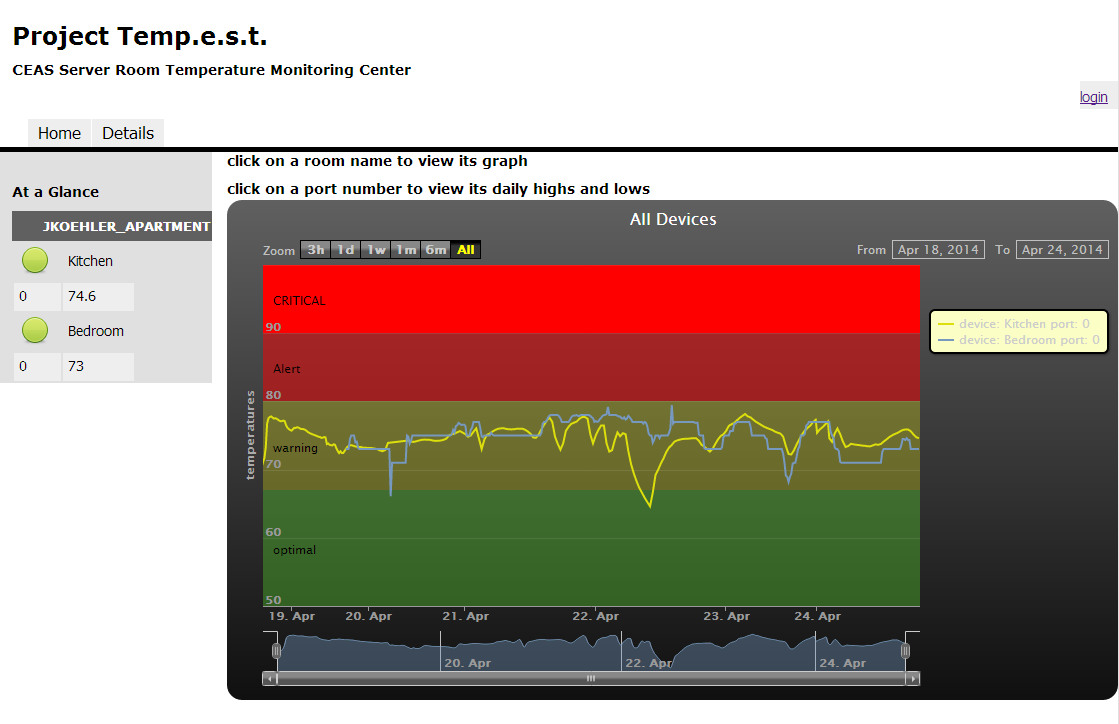
\includegraphics[scale=0.5]{Website.PNG}}
	\caption{Initial View Of Site}
\end{figure}
\indent
The main page of the website that we inherited from the previous team is shown above. On this page there is a graph of all the temperatures of reported by all the sensor units that are currently being tracked. It does not currently display any humidity readings. We will be evolving the site to include this information in future releases. The existing framework alloys easy data viewing with little programming effort. We will use the existing framework and expand the code to include humidity. Additionally, we will be adding additional graphing functionality using the logged historical data.
\newpage


\indent
The login process is very basic at this time. The existing web site uses lackluster security protocols, minimal, data sanitization, and no input verification. Our client has asked us to upgrade all security features and implement a system that will prevent session hijacking, network eavesdropping, cross site scripting, and brute force attacks.

\begin{figure}[H]
	\makebox[\textwidth]{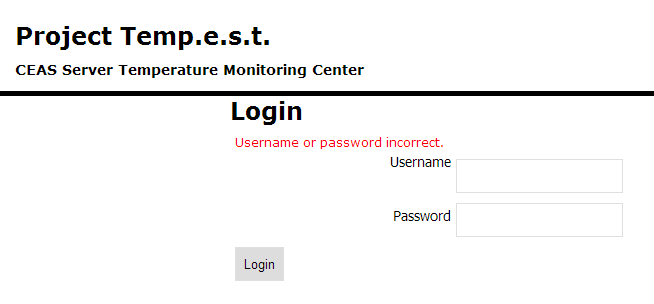
\includegraphics[scale=0.75]{LoginPage.PNG}}
	\caption{Login Page}
\end{figure}
\indent
As shown above, at this time the page has a simple “Username” and “Password” field along with a submit button. Our client has asked us to add additional features by adding a checkbox that disables the browser from remembering or saving this information. Our first “alpha” release will be using a test database with test users, test usernames, test passwords, and test data, so the security will not be an issue during this phase. When the user submits their credentials, the framework will reference the data to see if it matches what is in the database. If it does, the framework will provide further access to the site. If the authentication fails, the framework will require the user to try again. 
\newline
\indent
Our client asked us to create a single login page, but based on whether the user successfully authenticates as an administrator or a simple user provide the pages and views they have access to. The admin will have access to the identical pages as the user, but will have an administrator functionality added to the pages, which will allow them to add new users, rooms, and devices, as well as delete or modify existing users, rooms, and devices. A regular user will have a list of devices, whereas an administrator will see the same list but will have a button above said list that takes them to an “add device” page. The list will have an “edit” and “delete” button next to each device for administrators as well. The edit and delete pages will be similar to the add page, and will be basically the same for users, devices, and rooms.
\newpage

\begin{figure}[H]
	\makebox[\textwidth]{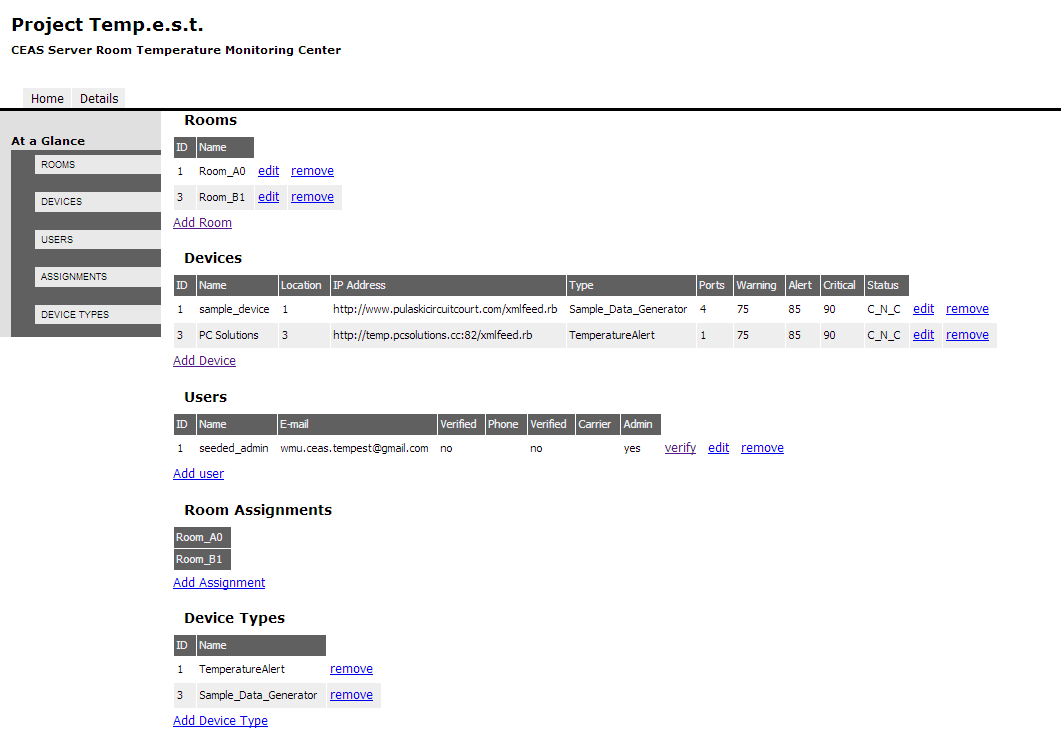
\includegraphics[scale=0.5]{AddPage.PNG}}
	\caption{Add Page}
\end{figure}
\indent
Upon logging in as a system administrator this is what the admin sees. This is the general hub for editing anything on the site. From here the admin can see rooms, users, room assignments and device types easily.
The page looks just the same for a room administrator when logging into the site. The only difference is that the room user won't have the option to edit any rooms, devices, etc. If a non logged-in user tries to access this page it redirects them to the login page so that all admin data isn't available to the public.
\newpage

\begin{figure}[H]
	\makebox[\textwidth]{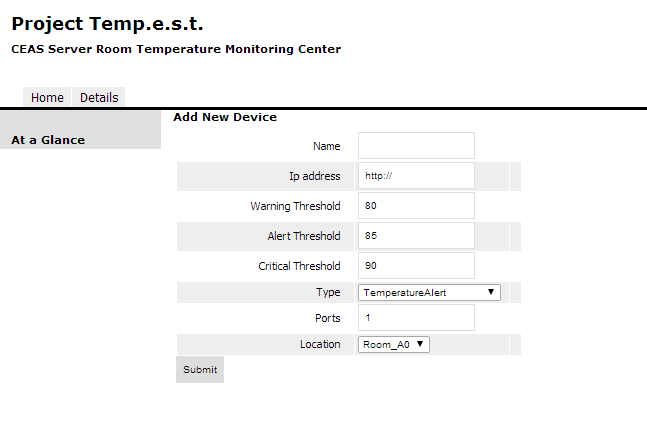
\includegraphics[scale=0.75]{AddDevice.PNG}}
	\caption{Add Device To Network Page}
\end{figure}
\indent
The above figure is the form used when adding a new device to the network. The IP address is a major need in this form because it tells the server where to look for the data. The alert and critical thresholds are for setting the threshold for when to warn administrators for that room. The number of ports specifies simply the number of temperatures to expect coming from that device.
\newpage

\begin{figure}[H]
	\makebox[\textwidth]{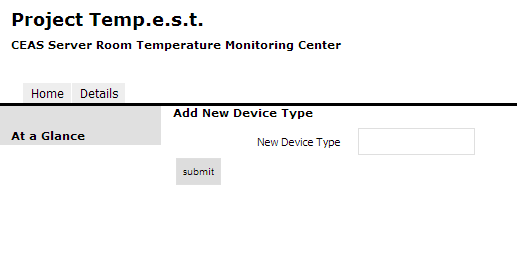
\includegraphics[scale=0.75]{AddDeviceType.PNG}}
	\caption{Add Another Device Type}
\end{figure}
\indent
The above page is used to add a room to the monitoring system. The main purpose of a room is to group sensors together and make it easier to distribute work among the administrators.
\newline
\indent
The below figure shows the page where a new room can be added.
\begin{figure}[H]
	\makebox[\textwidth]{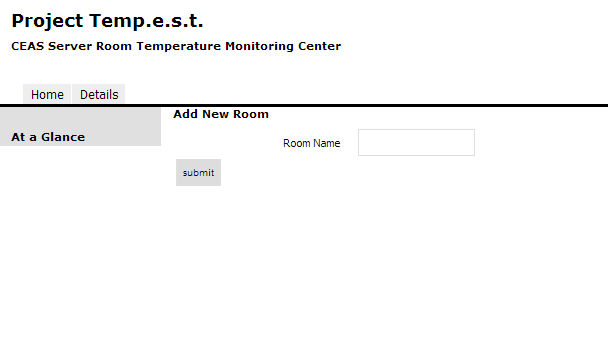
\includegraphics[scale=0.75]{AddRoom.PNG}}
	\caption{Adds a Room}
\end{figure}
\newpage

\indent
There are two different levels of users within the project. One level is the users and the higher level is the administrators.
\newline
\indent
The administrators are in charge of handling all room assignments as well as creating, updating and deleting users, devices, rooms and device types. These administrators also are able to be assigned to rooms just like a normal user.
\newline
\indent
The normal user can see the graph of data on the front page and login. They also receive alerts, but are not able to change any settings with the devices etc.
\begin{figure}[H]
	\makebox[\textwidth]{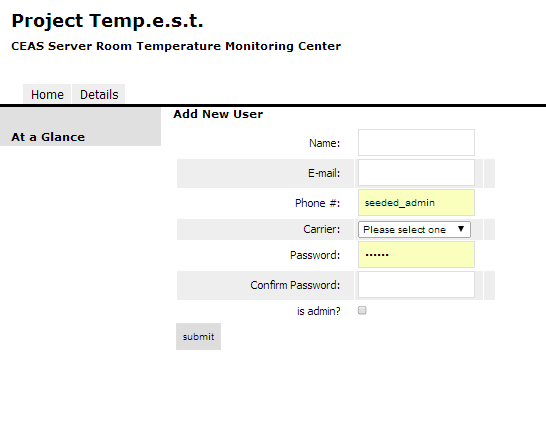
\includegraphics[scale=0.75]{AddUser.PNG}}
	\caption{Page To Add Users}
\end{figure}
\indent
Above is the form for adding a new user. The required fields are name, email, and password. The password does have minimal requirements for good passwords. This is not very secure, and the email is also unverified.
\newpage

\begin{figure}[H]
	\makebox[\textwidth]{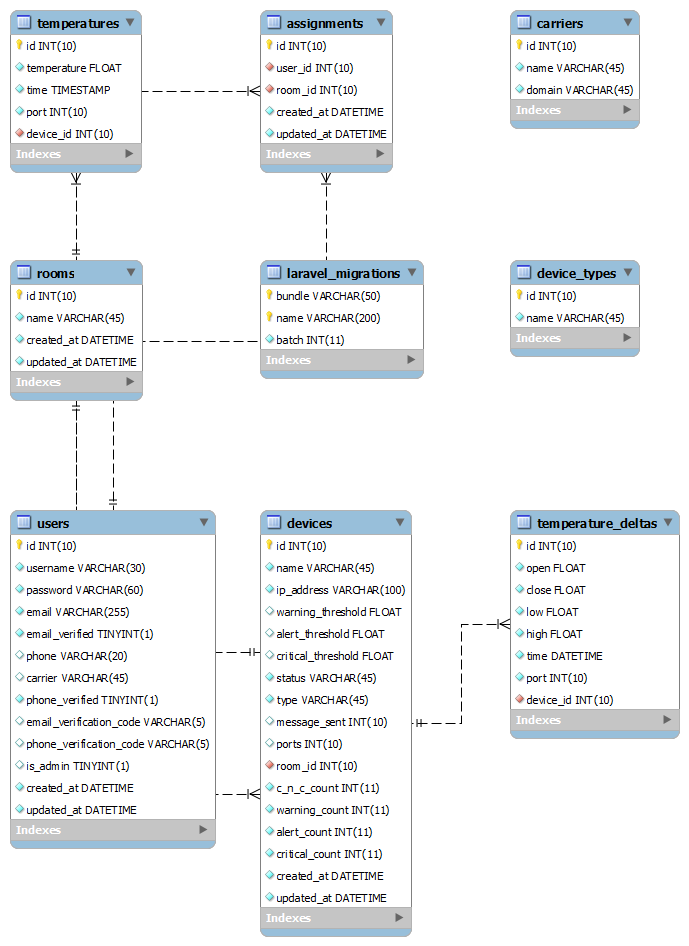
\includegraphics[scale=0.35]{ERDDiagram.png}}
	\caption{Entity Relationship Diagram}
\end{figure}
\indent
Above is the old database diagram of the web site. We decided to not make minor changes because the database was designed in a manner that didn't allow humidity recording without adding another table
\newpage

\subsection*{Design Decisions}
\addcontentsline{toc}{subsection}{Design Decisions}
\begin{center}
	\textbf{Hardware, The Microprocessor}
\end{center}
\indent
\indent
There were multiple options for microprocessors we could use. After some research, we narrowed down our list of possible units to these three: the RaspberryPi, the MSP430 Launchpad, and the Arduino Leonardo.
\newline
\begin{figure}[H]
	\makebox[\textwidth]{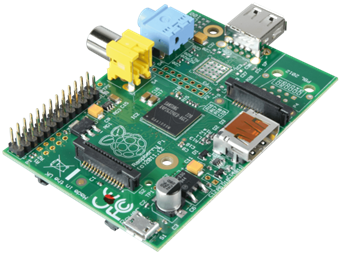
\includegraphics[scale=0.50]{raspberripi.png}}
	\caption{The RaspberryPi}
\end{figure}
\begin{figure}[H]
	\makebox[\textwidth]{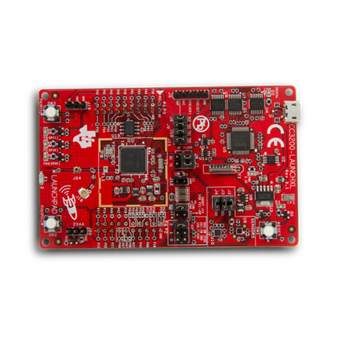
\includegraphics[scale=0.50]{msp430.png}}
	\caption{The MSP430 Launchpad}
\end{figure}
\begin{figure}[H]
	\makebox[\textwidth]{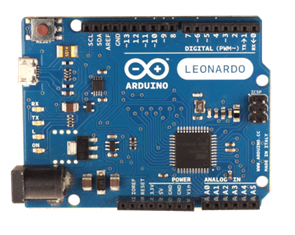
\includegraphics[scale=0.50]{arduino.png}}
	\caption{The Arduino Leonardo}
\end{figure}
\indent
Each of these devices had their own benefits. The MSP430 Launchpad was the cheapest option while the RaspberryPi was the most expensive option. A big problem with the MSP430 Launchpad is that is offers almost no features. It may be cheap, but the time, effort, and money we would need to put in to this device to connect it to the internet made it unusable to us.
\newline
\indent
The Arduino Leonardo was our second option. It came with many features. It was widely documented and widely used. But, the Arduino Leonardo face the same problem that the MSP430 Launchpad has: it isn't easily or cheaply connected to the internet.
\newline
\indent
Finally, the RaspberryPi. The RaspberryPi is heavily used and offers much documentation. In addition, it comes with multiple USB ports, an ethernet jack, and the ability to run a full Linux Operating System. This all comes in a \textdollar35 package. All we needed was to buy a \textdollar5 SD card to host the Operating System.
\newpage

\begin{center}
	\textbf{Hardware, The Sensors}
\end{center}
\indent
\indent
Our client asked us to use both temperature and humidity sensors. We found many sensors:
\begin{itemize}
	\item TMP36 Analog Temperature Sensor
	\item DS18B20 Digital Temperature Sensor
	\item AM2315 Digital Temperature Sensor
	\item DHT11 Sensor Unit
	\item DHT22 Sensor Unit
\end{itemize}
\indent
These sensor are all very good sensors in their own regard. We first looked at using two different sensors, and began by searching for temperature sensors.
\newline
\indent
The TMP36 was the first temperature sensor we looked at. It is cheap, and fast. It's also analog. Because it is an analog sensor, it requires calibration for each individual sensor. This is too much work and can cause reliablitiy issues, so we did not go with the TMP36.
\newline
\indent
The DS18B20 and AM2315 sensors were the next sensors we looked at. Both are digital, and require no calibration. We immediately removed the AM2315 from our list because it costs \textdollar30. We purchased a few DS18B20 sensors to do some preliminary testing. It is slow, requiring about a second to return proper data.
\newline
\indent
As we'd found our temperature sensor, we began looking for a humidity sensor. All of the ones we found received terrible reviews and we ignored them altogether. Then, we stumbled upon the DHT11 Sensor Unit. This sensor reads both temperature and humidity and is digital. It is about 3 times more expensive than a DS18B20 but is just as slow.
\newline
\indent
After testing for a few weeks, we began looking at the accuracy of our DHT11. As it turns out, the DHT11 is about 4 times worse in terms of accuracy than the existing \textdollar300 Temperature@lert units in place. We soon found out that the DHT11 has a big bother, the DHT22. It performs the same functions as the DHT11, but has a wider range of sensing, and is just as accurate as the existing Temperature@lert units. While the DHT22 is \textdollar5, it is very powerful and inscredibly accurate, and we decided to use the DHT22 for our final sensor.
\newpage

\begin{center}
	\textbf{Hardware, Enabling Internet Connectivity}
\end{center}
\indent
\indent
We had two options for connecting our RaspberryPi sensors to the internet: a wireless or a wired connection. Both options we available to us by our Client.
\newline
\indent
Using the wired connection approach, we would be able to run the RaspberryPi using Power-over-Ethernet(PoE). All of WMU's ethernet cables in the CEAS building are PoE capable. The problem with this approach is the RaspberryPi doesn't allow PoE. We would need a PoE splitter attached to the RaspberryPi to remove the power from the ethernet cable and convert is to USB power which the RaspberryPi accepts. The benefits of PoE is that the RaspberryPi would not need an AC power unit.
\newline
\indent
Another drawback of using a wired connection would be the need to run an ethernet cable to wherever the RaspberryPi will be located. This is very inconvenient for moving the sensor units around and for cable cleanliness in general.
\newline
\indent
In contrast, using a wireless connection opens us up to a wide range of uses. While the USB wireless unit does cost about \textdollar10, this was a cost we were willing to incur. The wireless adapter we chose is a generic 802.11n adapter, but it is backwards compatible with the 802.11a/b/g protocols. Using a wireless adapter, we can move the sensor unit around to any location we require it to be, and because the 802.11n protocol is a long range protocol, we can go quite a distance from a wireless internet access point.
\newpage

\begin{center}
	\textbf{Software, Web Framework}
\end{center}
\indent
\indent
For our web framework, we had many choices. We had options ranging from Ruby on Rails, to Tomcat, to CakePHP, and even to code in raw PHP without a framework. In the end, we decided to use Laravel. We did extensive research, and found, according to the graph below, that Laravel has the most market share of all PHP web frameworks.
\begin{figure}[H]
	\makebox[\textwidth]{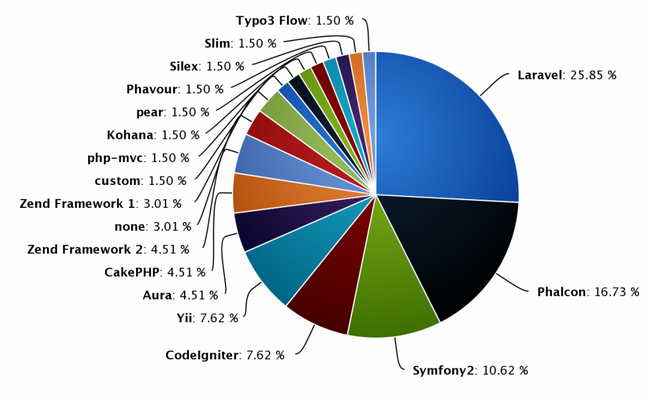
\includegraphics[scale=0.75]{frameworks2.png}}
	\caption{The Market Share of PHP Web Frameworks}
\end{figure}
\indent
Having over a quarter market share over all other PHP web frameworks means that Laravel is doing something right. It also means that people trust Laravel, and because of this, there is quite a lot of documentation.
\newline
\indent
We did have a few more specific reasons for choosing Laravel over our other options. One of the biggest reasons we chose Laravel is because it has industry-standard security measures, that, when implemented properly, can lead to a very secure web site. In addition, Laravel is a little older, and has had time to mature and work out bugs. Therefore, Laravel provides an incredibly reliable Model-View-Controller system. As an added bonus, it's even open source!
\newpage

\begin{center}
	\textbf{Software, Sensor Unit Programming Language}
\end{center}
\indent
\indent
Our RaspberryPi sensor unit requires some form of programming language. This decision should have been a rather simple decision, but during test, we had some issues. The manufacturer of our DHT22 sensing unit provides libraries for us to use to interface with the DHT22. During testing, we had some problems occur while trying to read data off of the DHT22. Originally, we used the C programming language to write the code which reads the DHT22. While C is incredibly fast, it requires compilation, which turns out wasn't the worst of our issues. While polling the DHT22 for measurements, it took the program anywhere from one to 15 tries to properly read the data. In our eyes, that isn't very reliable.
\newline
\indent
We decided to give Python a try. Python is a slow language but it doesn't require compilation. It is also extremely reliable, as the program we wrote reads the measurements properly the first time, every time. While it is slow, waiting about two seconds for an updated measurement is something our client was willing to live with, as the propagation of that data to the user-facing front end still takes time, and waiting an extra few seconds will not impact any hardware any more.
\newpage

\begin{center}
	\textbf{Server}
\end{center}
\indent
For our server setup, we had to make a few decisions.
\begin{itemize}
	\item What Operating System should we use?
	\item What Web Server should we use?
	\item What Database technology should we use?
	\item What Framework should we use?
	\item Where do we host the web server?
\end{itemize}
\indent
These questions are all equally important. We first had to pick the Operating System. We had the choice between Windows, a rather expensive option, and Linux, a very free option. We decided to go for the Linux system because of the cost and because it is open source.
\newline
\indent
Once we had our Operating System chosen, we made the decision to use a set of technologies that are very commonly used. It's called a LAMP stack, and stands for Linux, Apache, MySQL, and PHP. We had other options for each of these technologies. We could have used a web server called nginx, but the documentation and historical evidence of Apache working was already there. There were other database technologies that we could have used, but MySQL is free, powerful, and well documented. Finally, our reasoning behind PHP was explained in the Web Framework Design Decisions.
\newline
\indent
Finally, we had to choose where we wanted to host our website. We had options available to use like Microsoft Azure, Linode, or DigitalOcean. We opted for Amazon Web Services(AWS).
\newline
\indent
Our primary reason for picking AWS was that it is free for the first year, and then only \textdollar10 per month. In addition, we can easily migrate our virtual machine with great ease, and the uptime for any AWS service is more than 99.95\%. As an added bonus, AWS gives us unlimited bandwidth at no extra charge. Even though our web site and server doesn't use much data at all, a heavy user load can add up quickly.
\newpage

\begin{center}
	\textbf{Web Site, Design and Styling}
\end{center}
\indent
\indent
The existing web site that we took over from the previous team did not look nice at all. The buttons were ugly, the styling was poor, and the colors were mismatched. Furthermore, it was not mobile-compatibly at all. We had to find a solution.
\newline
\indent
We decided to tackle the graphs on the pages first. The existing web site used High Charts, which is a rather useful graphing library. As it turns out, the version that was being used was quite outdated. We updated it, and most of the problems that existed were gone. The updated version provided mobile support, scaled well, and looked much cleaner.
\newline
\indent
There were alternatives for us to use. We could have scrapped High Charts altogether and gone with commonly used libraries like Google Charts, or Chart.js. We also thought about using the YUI, the Yahoo User Interface Library. All of these are used often across many different implementations, but we decided to stick with High Charts because it worked and provided all the functionality we required without a massive re-write of the main pages.
\newline
\indent
Along with an updated and cleaner charting library, we decided to scrap most of the existing styling on the web site. We wanted our web site to be accessible across all devices, and the existing site didn't provide that. We looked at using jQuery Mobile, which can be slow, and Foundation, which is not insanely popular. We opted to go with a library called Bootstrap. Bootstrap is open source, widely used, and well documented. It's also incredibly easy to use and modify. One of our group members also had extensive experience using Bootstrap which contributed greatly to this choice as well. Bootstrap relies on a basic set of class tags which propagate and scale incredibly well. Once we finished implementing Bootstrap, the website became usable on any device and looked really nice.
\newpage

\subsection*{Design}
\addcontentsline{toc}{subsection}{Design}
\indent
\indent
Next we shall look at how the pieces interact with each other to create the system. First we will look at an overview of how the server, the user and the devices interact and how they are setup. 
\newline
\indent
On the right of the figure below, we have different rooms that are set up. Each room has sensors in it of any type. Each sensor hosts an xml document that shows the current information about the sensor. The central management server then on a routine basis will go out and fetch data from these sources and respond accordingly ie text or email if a threshold has been reached. The user can also view the website and it will interact with the user appropriately that way.
\begin{figure}[H]
	\makebox[\textwidth]{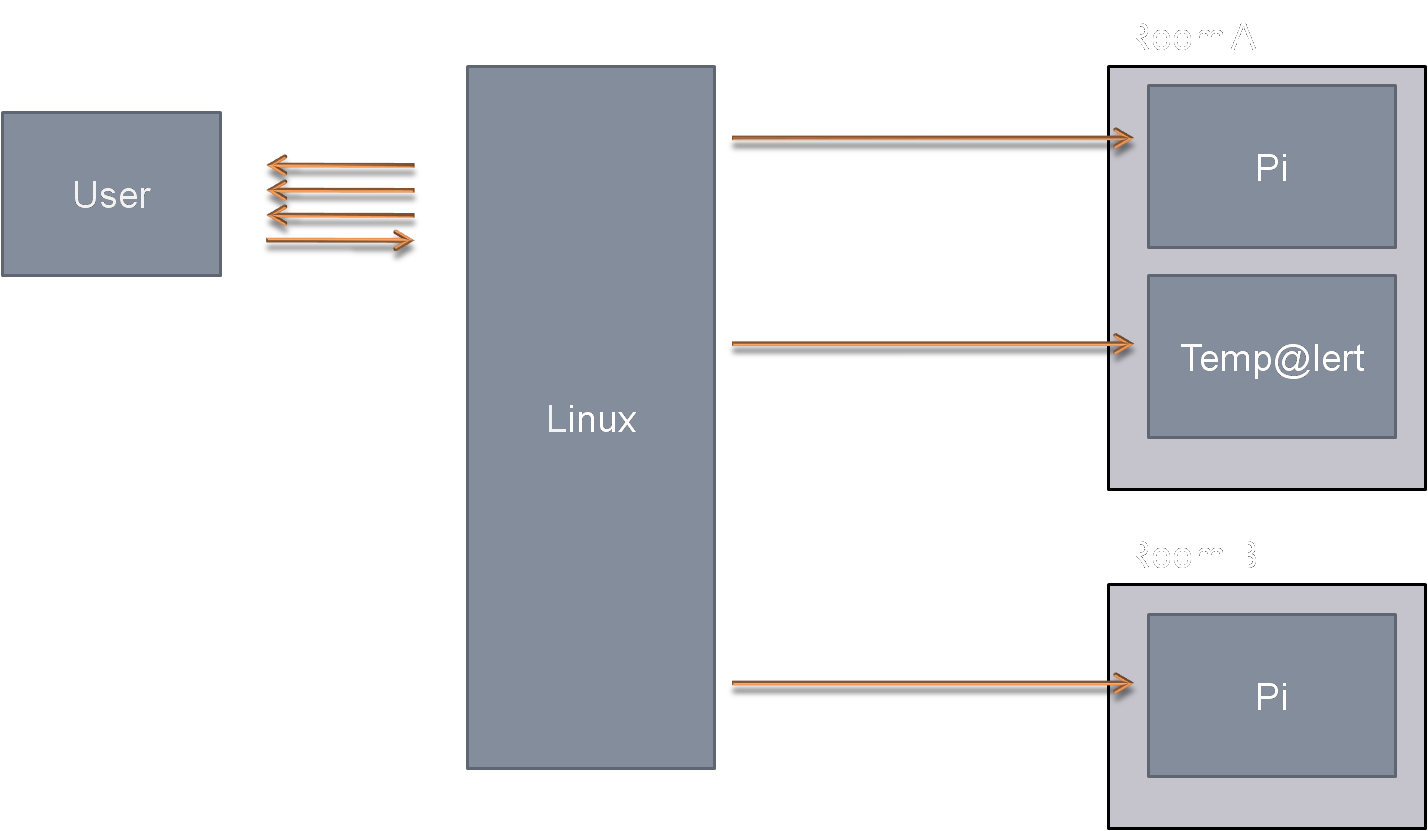
\includegraphics[scale=0.75]{overlook.png}}
	\caption{Overlook of the User, Server, and Device Relations}
\end{figure}
\begin{figure}[H]
	\makebox[\textwidth]{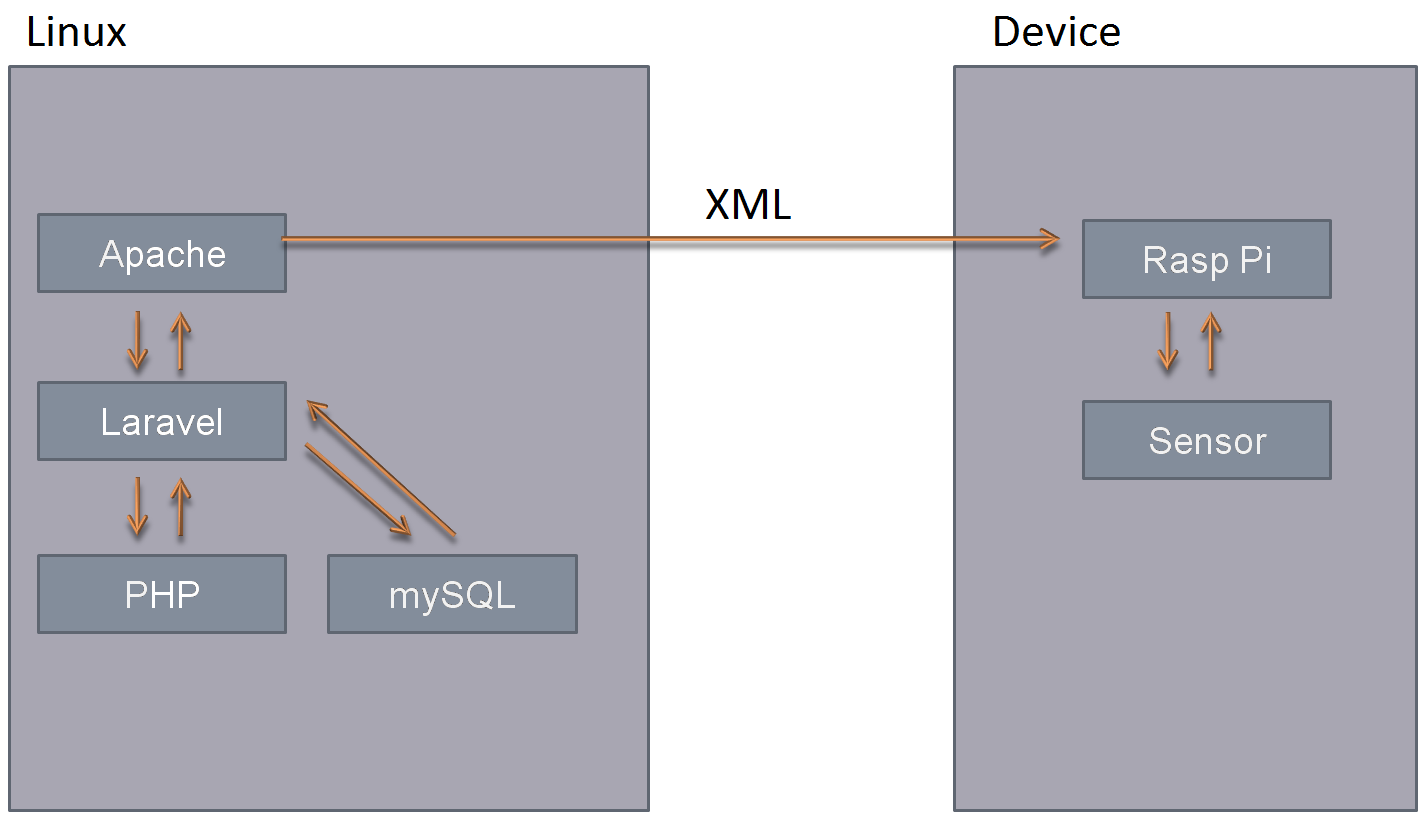
\includegraphics[scale=0.75]{zoomed.png}}
	\caption{Closer Look of Server and Raspberry Pi}
\end{figure}
\indent
Now to take a closer look at the interactions between the custom built raspberry pi sensing unit and the Linux central management system. On the Linux side we have the LAMP stack. Our laravel framework depends on this stack to function appropriately. When the time comes laravel will need to update the current temperature that a device has. So it will download the XML file from the device and send it through the driver for that device type. After that it will store the data in the database and based on the constraints for that device determine what the status of the device is and if it needs to react to its temperature. 
\newline
\indent
Meanwhile on the RaspberryPi side we have the RaspberryPi communicating with the sensor. The frequency of how often the sensor unit should be polled is determined by the administrator when the device is first set up. This is created through as simple cron job.After data has been polled the program writes it to an XML file that is hosted by apache on the RaspberryPi. For a more detailed description of how the RaspberryPi interacts with the sensors, please see the  
\newpage

\subsection*{Implementation}
\addcontentsline{toc}{subsection}{Implementation}
\indent
\indent
Now how did this design turn out. Before all the old site vital areas were shown. Now after implementing BootStrap we have a completely different front end. Here is the initial view of the site once a user has logged in.
\begin{figure}[H]
	\makebox[\textwidth]{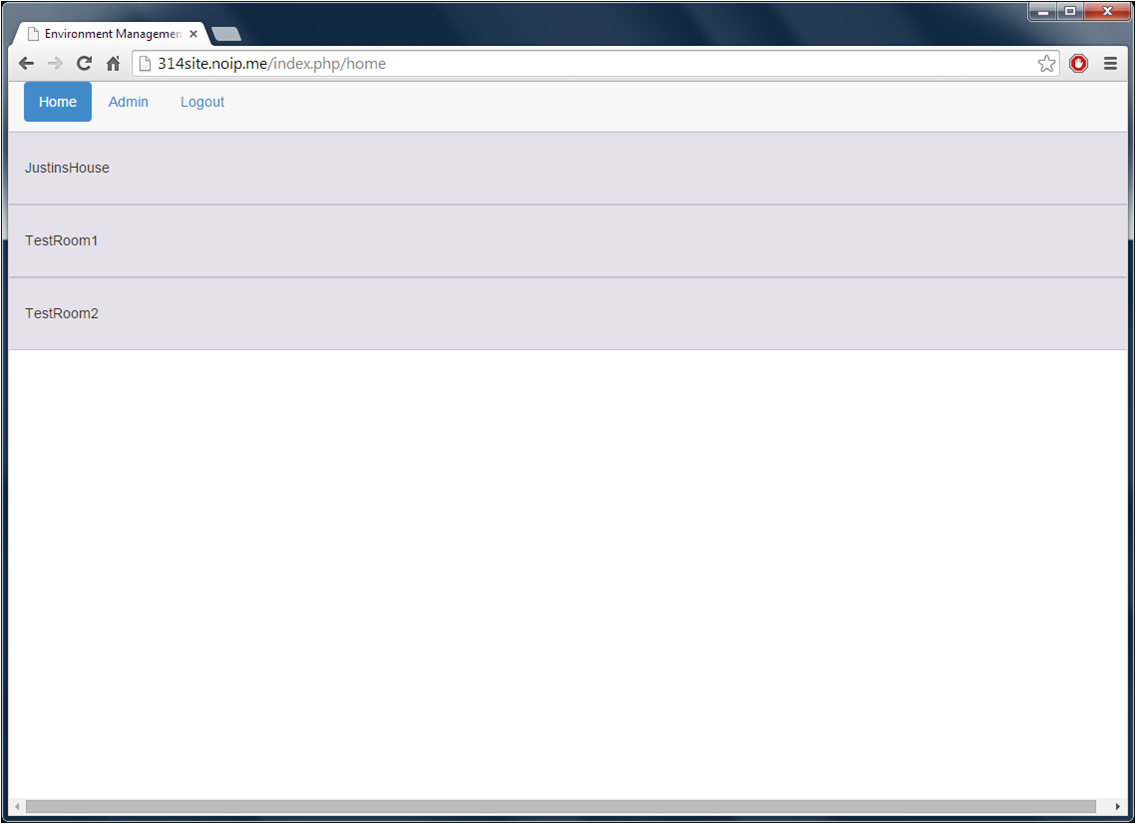
\includegraphics[scale=0.75]{firstlogin.PNG}}
	\caption{After Logging In on a Desktop Computer}
\end{figure}
\newpage

\indent
Now when a user clicks on the tab it will expand to show what the current temperature and humidity are. Next to that is the status of the machine i.e. okay or critical. Upon mousing over the graph it will give the temperature or humidity at that time in history. See the next figure.
\begin{figure}[H]
	\makebox[\textwidth]{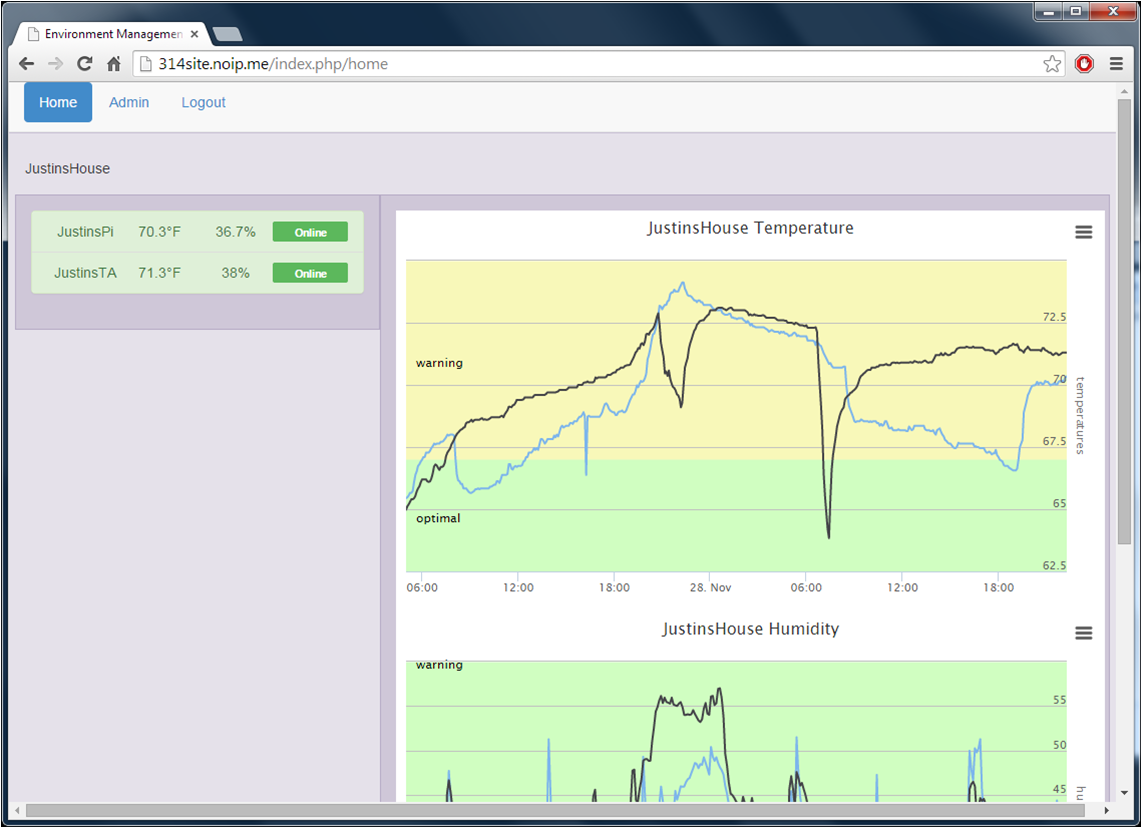
\includegraphics[scale=0.75]{opentabfirst.PNG}}
	\caption{Open Tab and Data}
\end{figure}
\newpage

\indent
These tabs are the same for each room and will show all appropriate data for each room. Next is the new and improved administration panel. On this panel there are five different tabs rooms, devices, users, room assignments and device types. All of these different devices the administrator is able to create, update and delete anything in those tabs. 
\begin{figure}[H]
	\makebox[\textwidth]{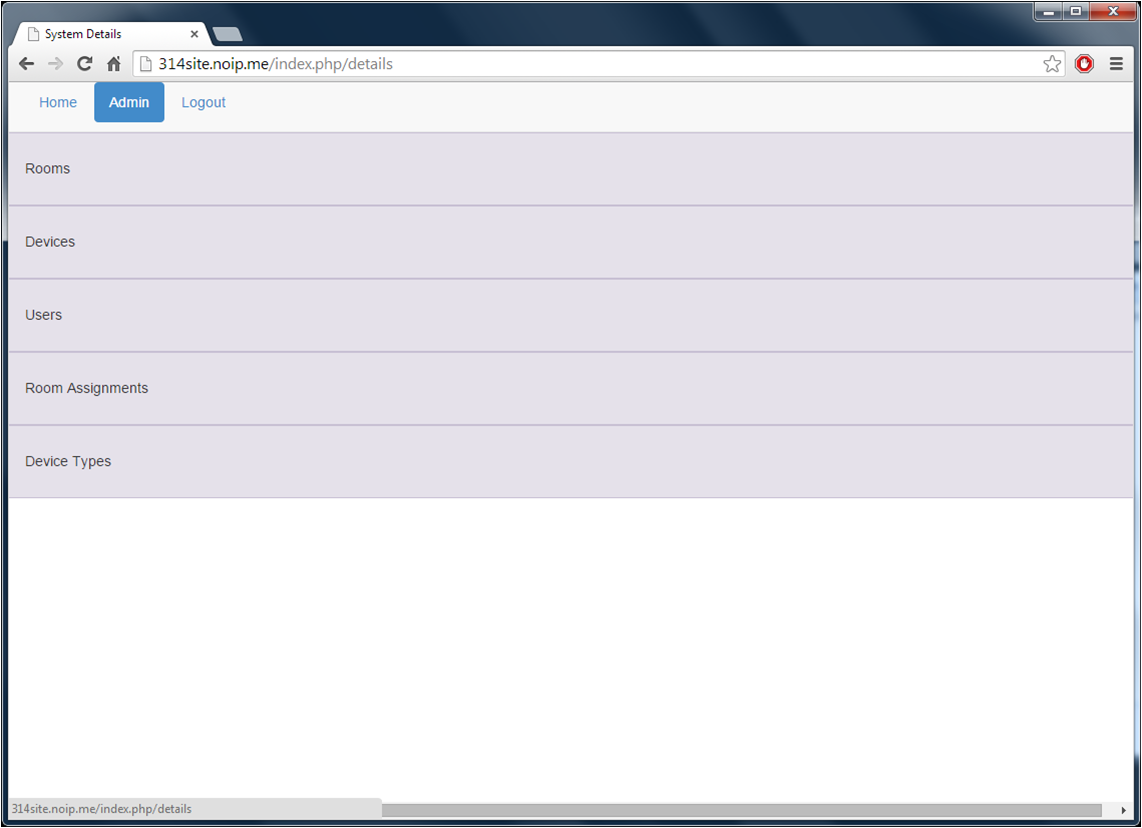
\includegraphics[scale=0.75]{adminpaneldesktop.PNG}}
	\caption{First View of Administration Panel}
\end{figure}
\newpage

\indent
The rooms tab has just those options and only has room name as its only parameter. See the next figure for the rooms user interface.
\begin{figure}[H]
	\makebox[\textwidth]{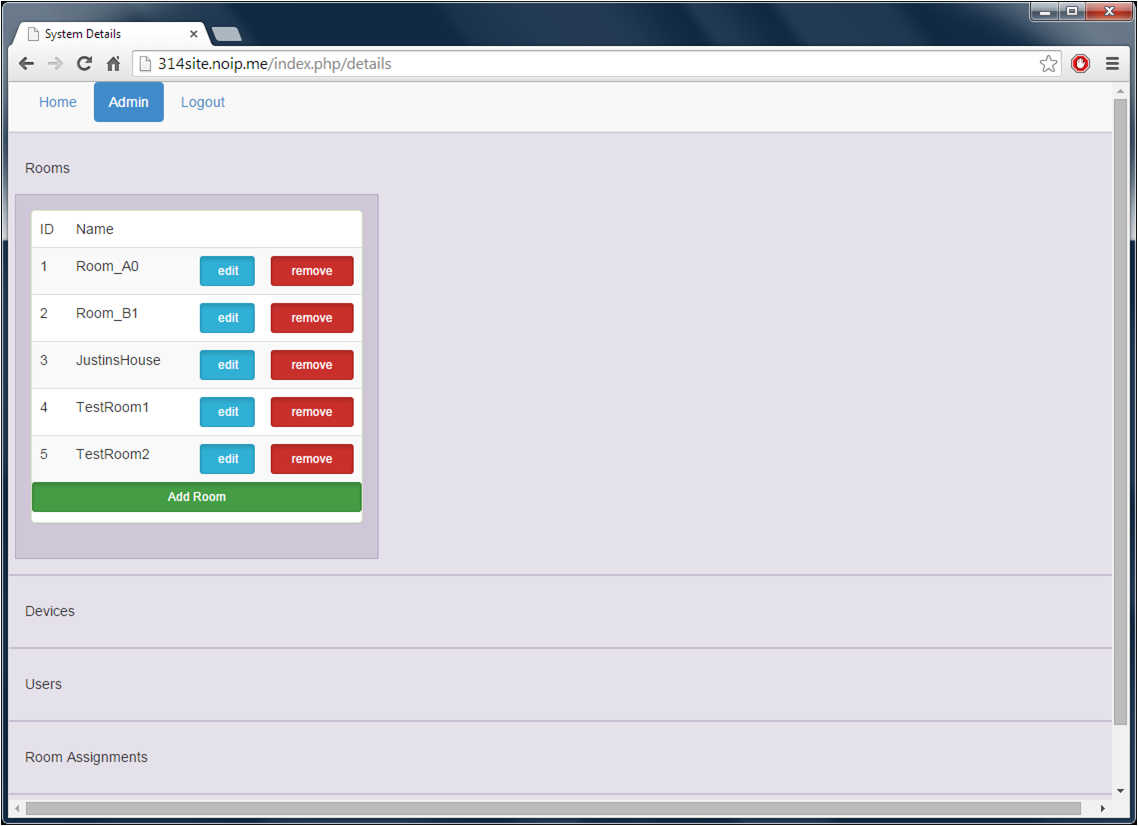
\includegraphics[scale=0.75]{roomsdesktop.PNG}}
	\caption{View of the Rooms Tab}
\end{figure}
\newpage

\indent
The next tab devices tab. This tab shows the device id, name, location, ip address, type of device, number of ports on the device, warning, alert and critical temperatures, and lastly status. The administrator can add, remove and update devices. 
\begin{figure}[H]
	\makebox[\textwidth]{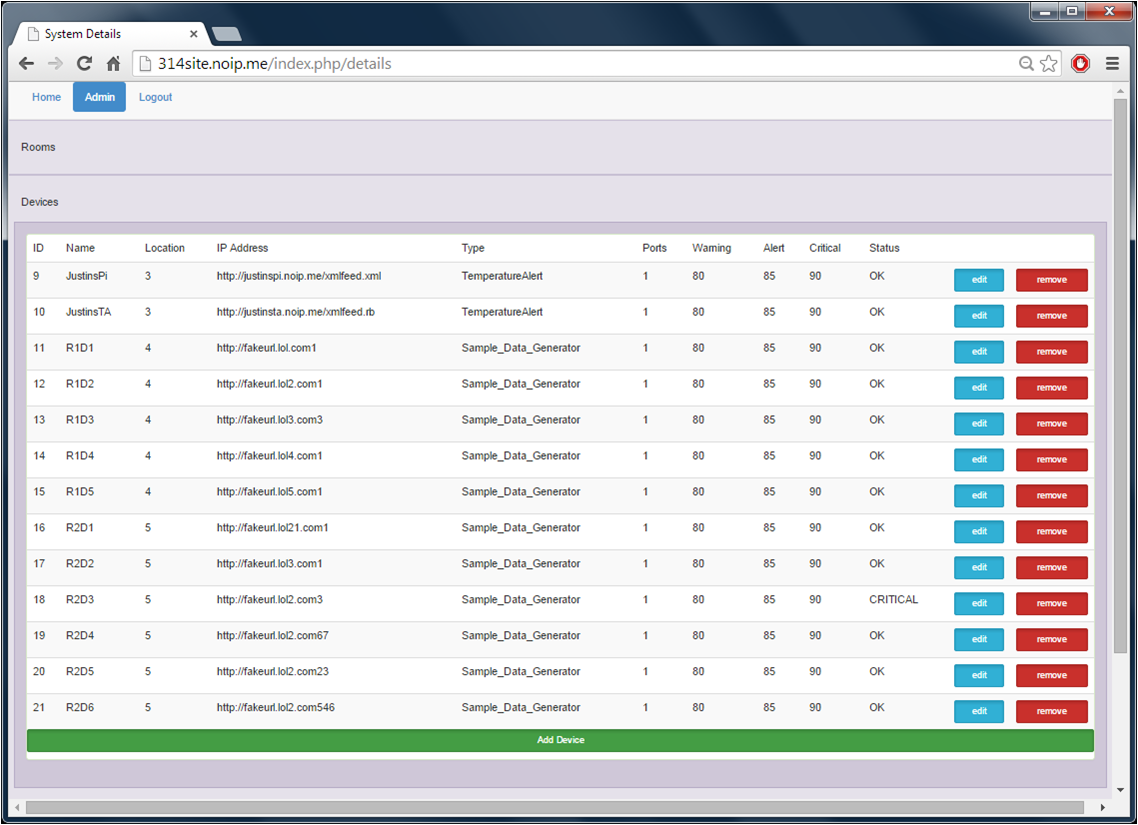
\includegraphics[scale=0.75]{devicesdesktop.PNG}}
	\caption{Device Administration}
\end{figure}
\newpage

\indent
The users tab allows new users and administrators to be created as well as updating and deleting users. This tab also allows verification of the users email and phone alerts. For a verification the user receives a text or email with a verification code that that the user types in the code and this allows the system to verify that the text or email went through.
\begin{figure}[H]
	\makebox[\textwidth]{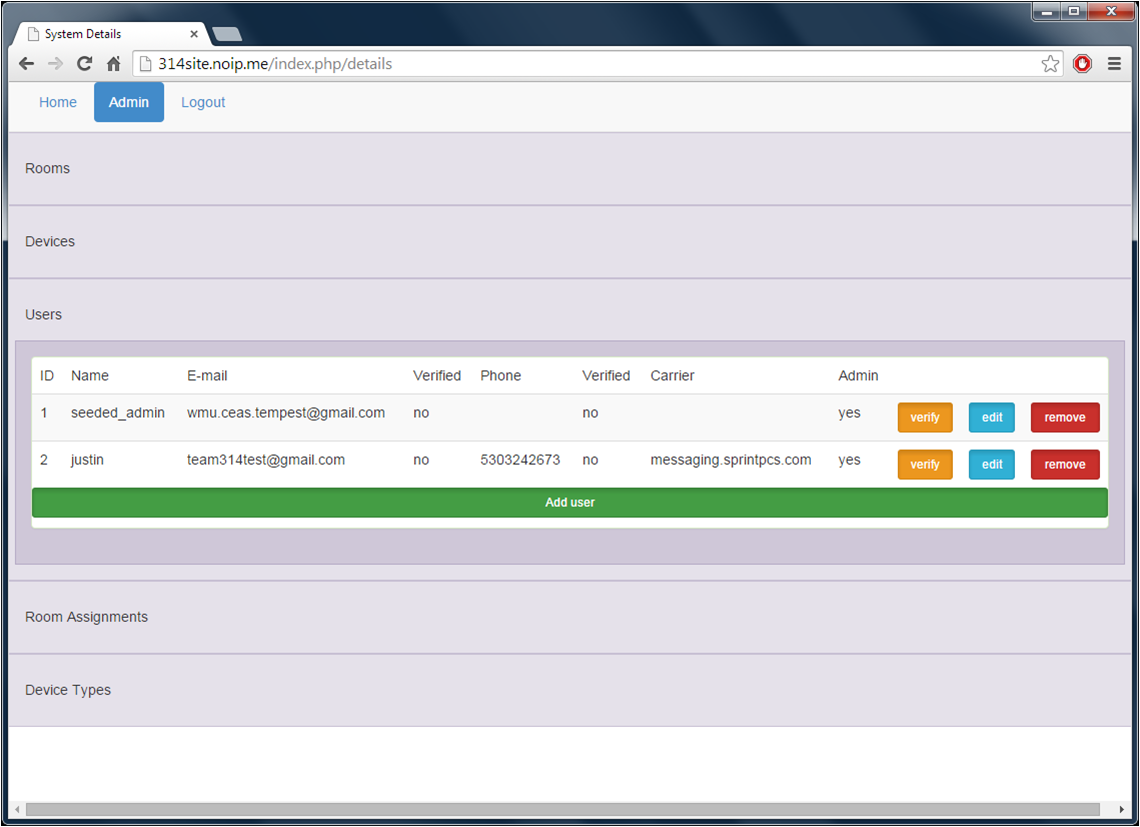
\includegraphics[scale=0.75]{usersdesktop.PNG}}
	\caption{User Administration}
\end{figure}
\newpage

\indent
The room assignments tab is very important. This is where administrators assign users to rooms. When a user is assigned to a room they will receive alerts when temperature benchmarks are reached.
\begin{figure}[H]
	\makebox[\textwidth]{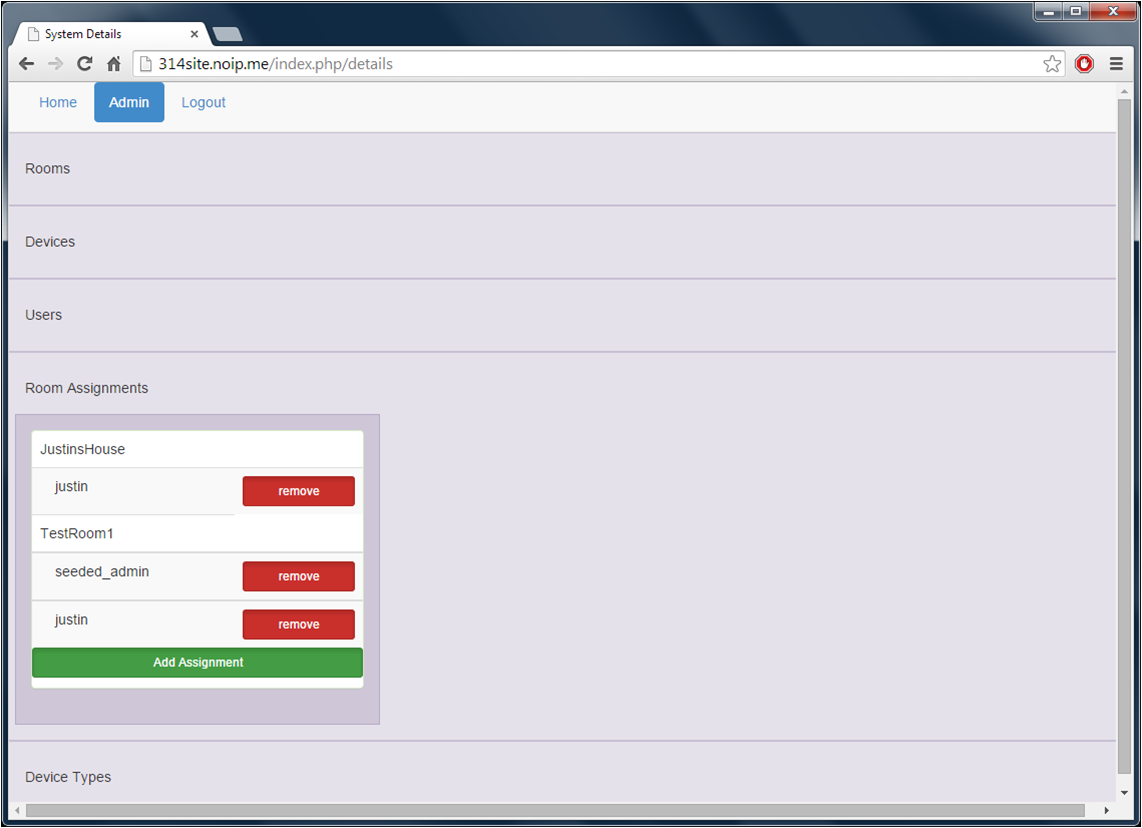
\includegraphics[scale=0.75]{roomassignmentsdesktop.PNG}}
	\caption{User Room Assignments}
\end{figure}
\newpage

\indent 
The last piece of the administration panel is the device tab. This device type tab. This is where the administrator can add different types of devices based on what they want to connect to their system. We have two device drivers that we have created. One is for the temperature @lert system which our raspberry pi also uses, and we have one for test sensors. If someone wanted to create their own driver they would make the connection here between the ui and the driver and then would need to create a driver to parse the XML.
\begin{figure}[H]
	\makebox[\textwidth]{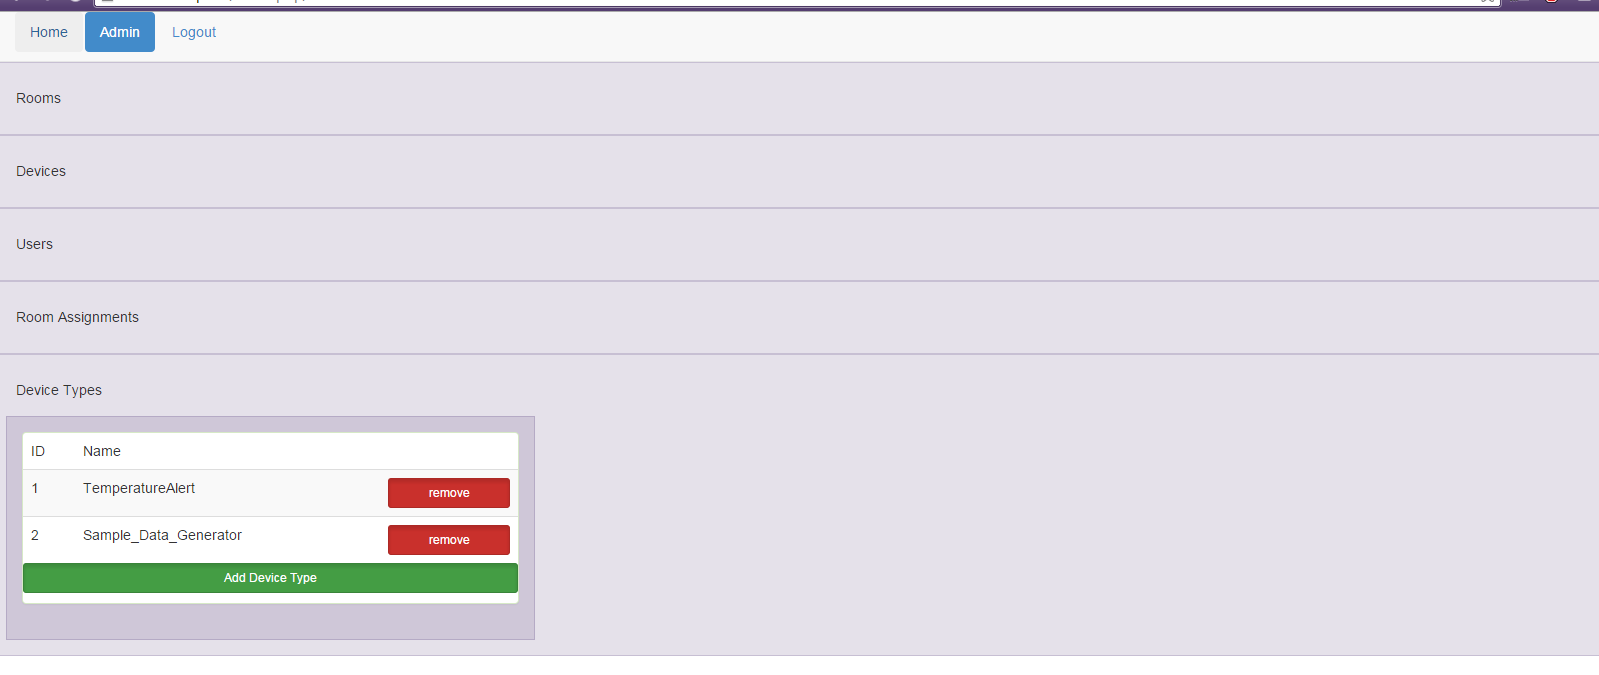
\includegraphics[scale=0.45]{Devicetype.PNG}}
	\caption{User Room Assignments}
\end{figure}
\newpage

\indent
One important feature that the client said was a must is that there must be support for mobile devices as we have stated before. The website on a mobile device looks almost identical to the desktop version of the site. Below are some screen shots from mobile devices looking at normal pages in the temperature window and the administration panel.
\begin{figure}[H]
	\makebox[\textwidth]{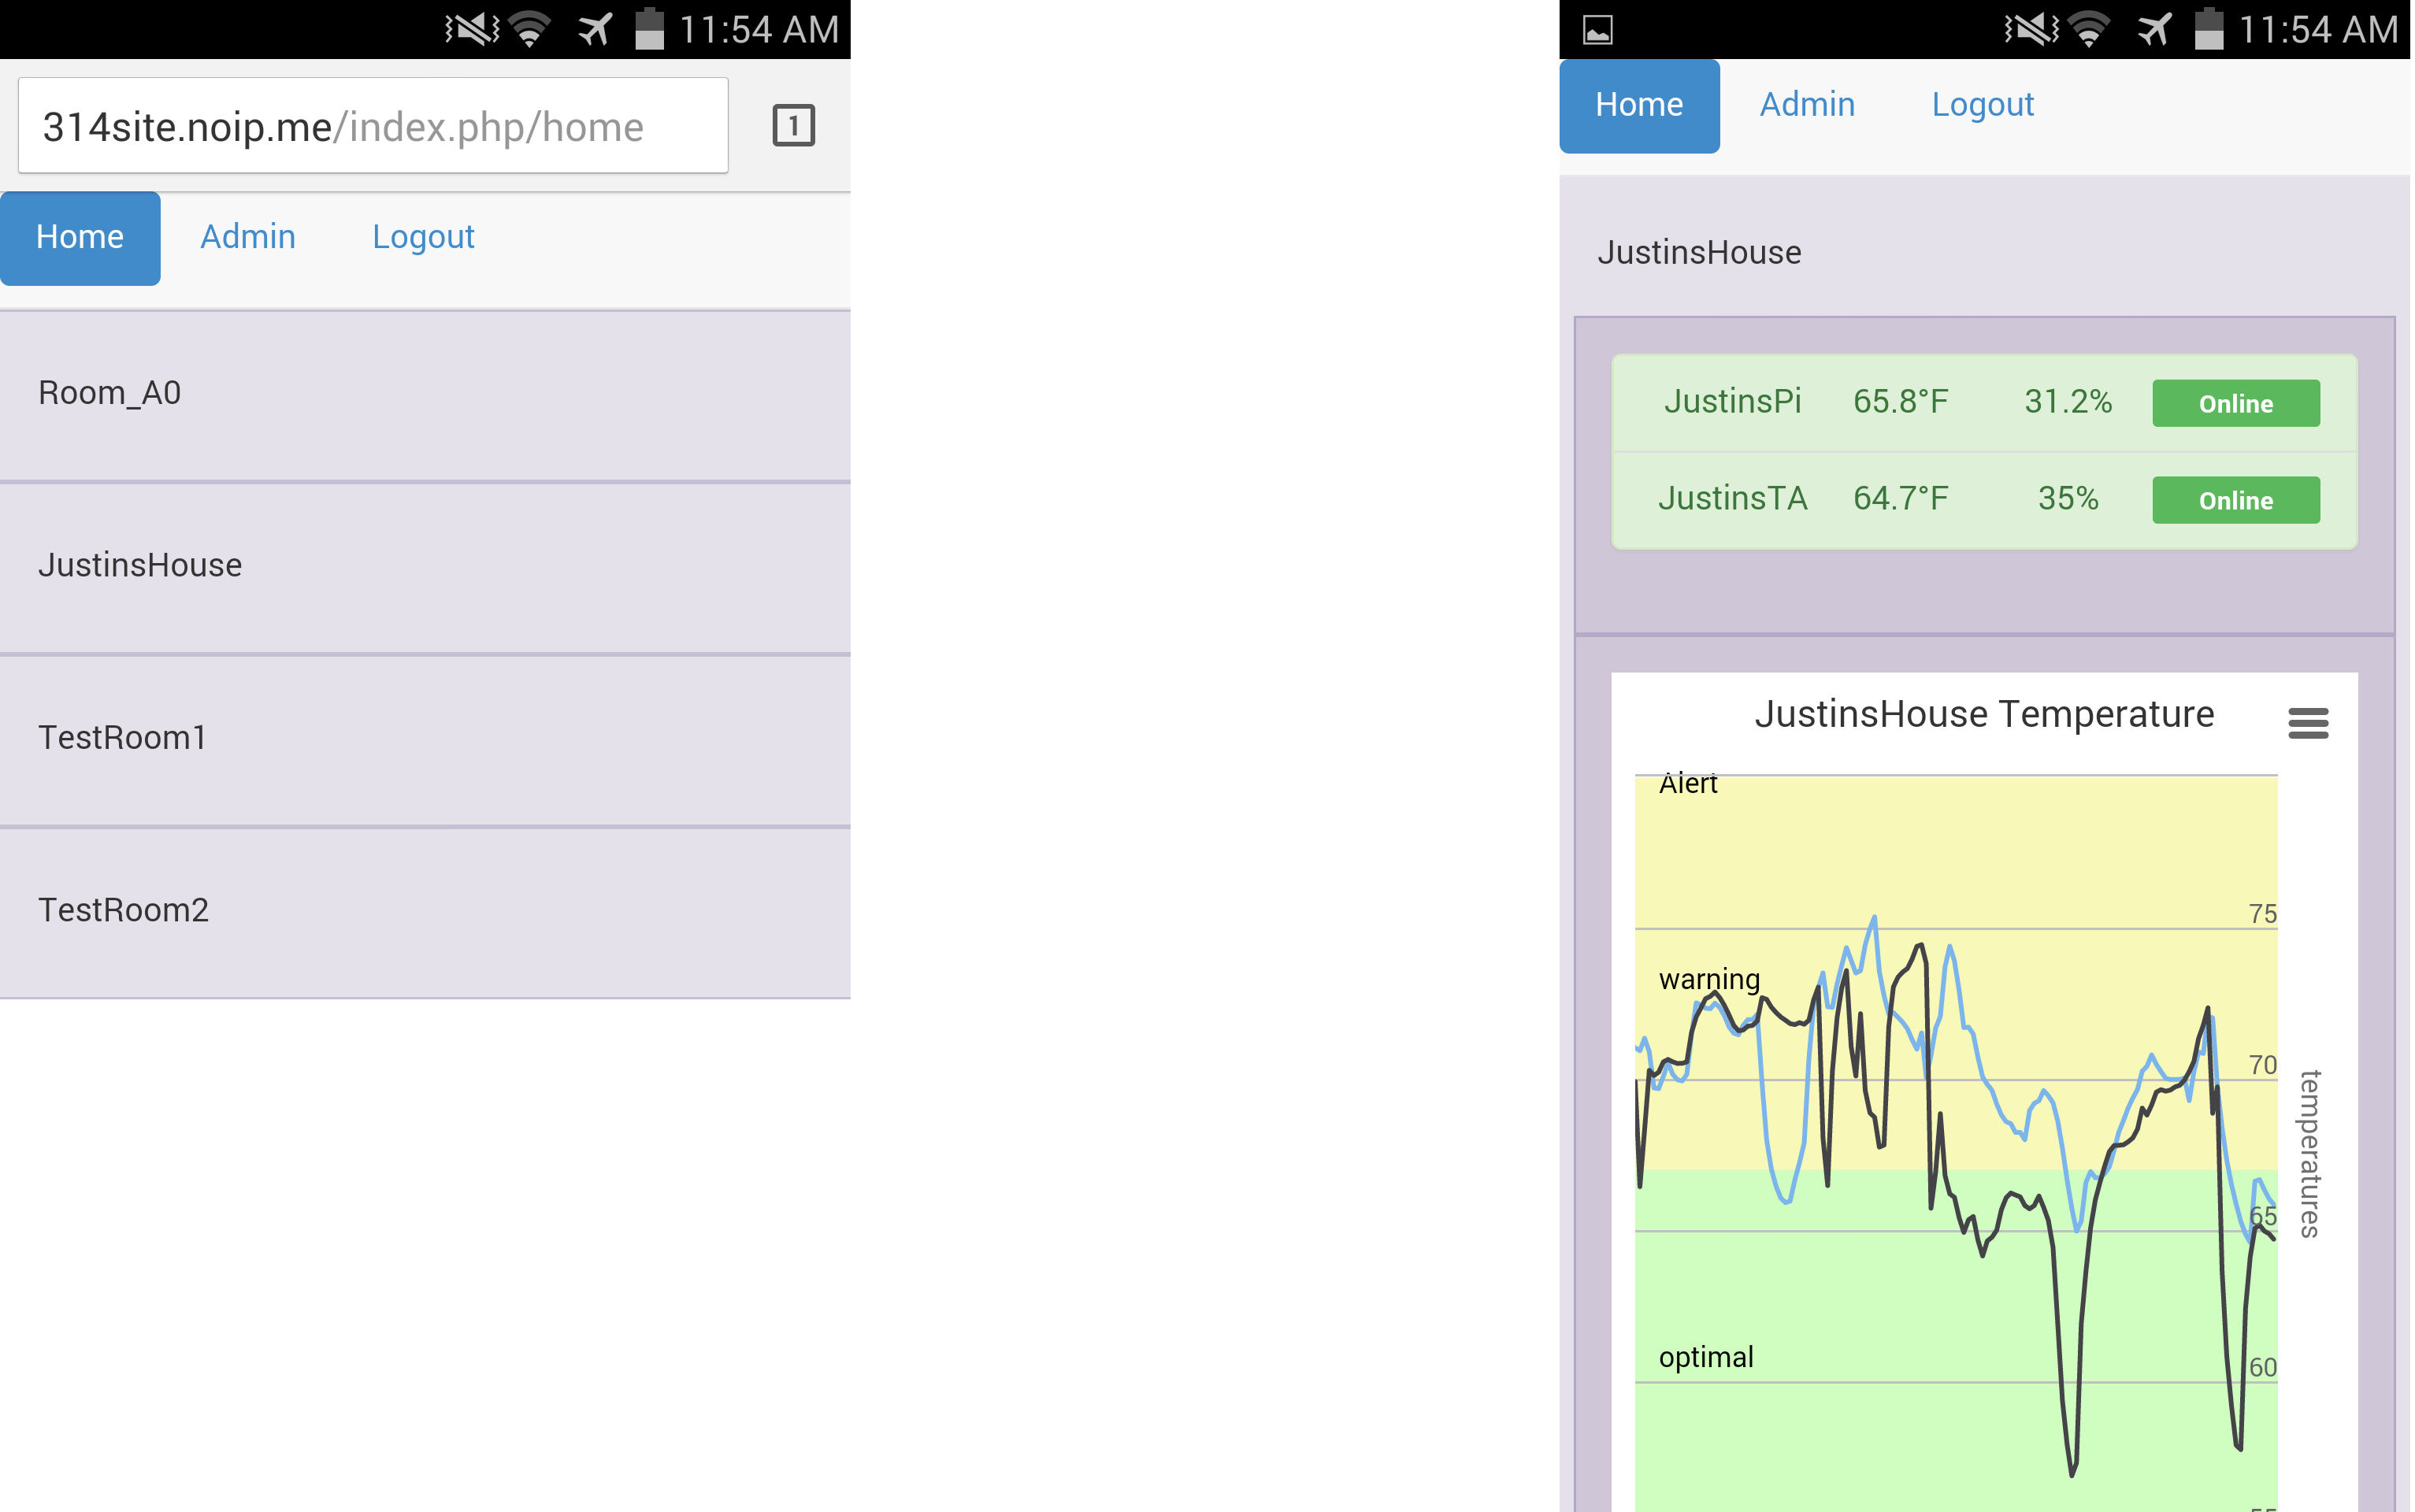
\includegraphics[scale=0.25]{mobilecombined.PNG}}
	\caption{User Area On Mobile Device}
\end{figure}
\begin{figure}[H]
	\makebox[\textwidth]{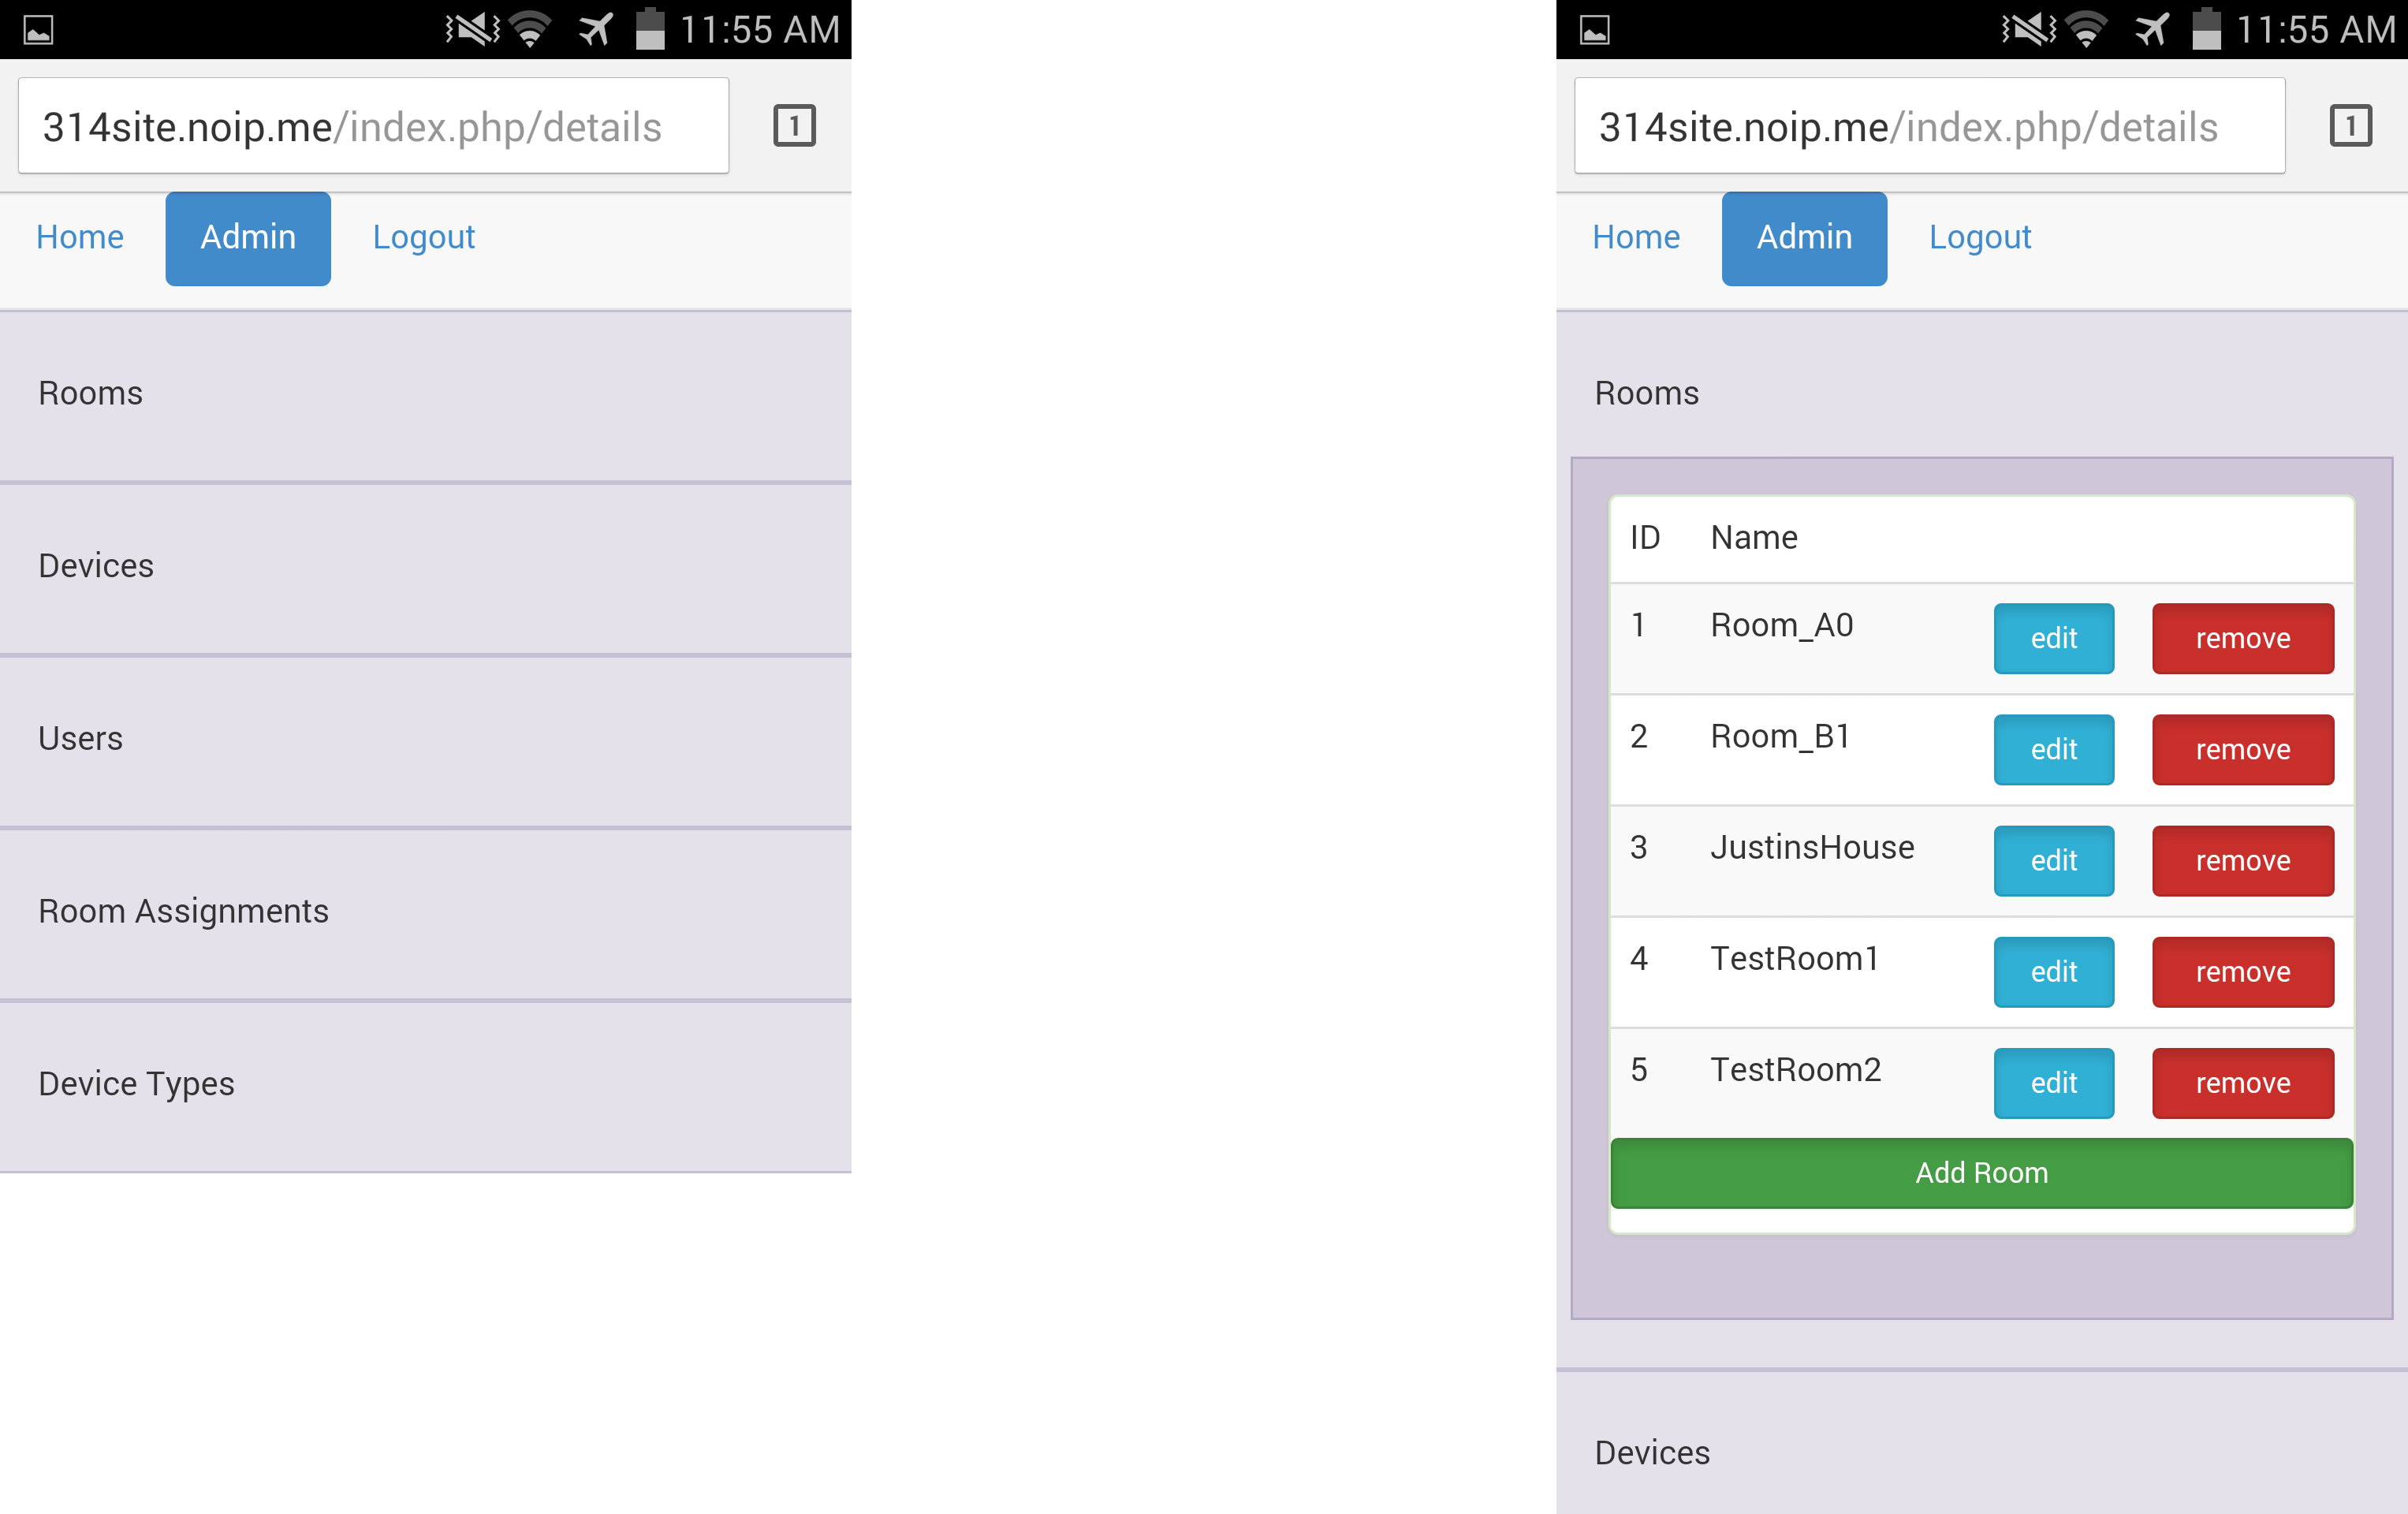
\includegraphics[scale=0.25]{mobilecombinedadmin.PNG}}
	\caption{Administration Panel on Mobile Device}
\end{figure}
\newpage

\indent
Now that the new site has been shown we will take a look at the finished product of the raspberry pi. First we have a picture of the device not assembled. There is the white temperature sensor, the black sd card, the usb wireless adapter and lastly the raspberry pi.
\begin{figure}[H]
	\makebox[\textwidth]{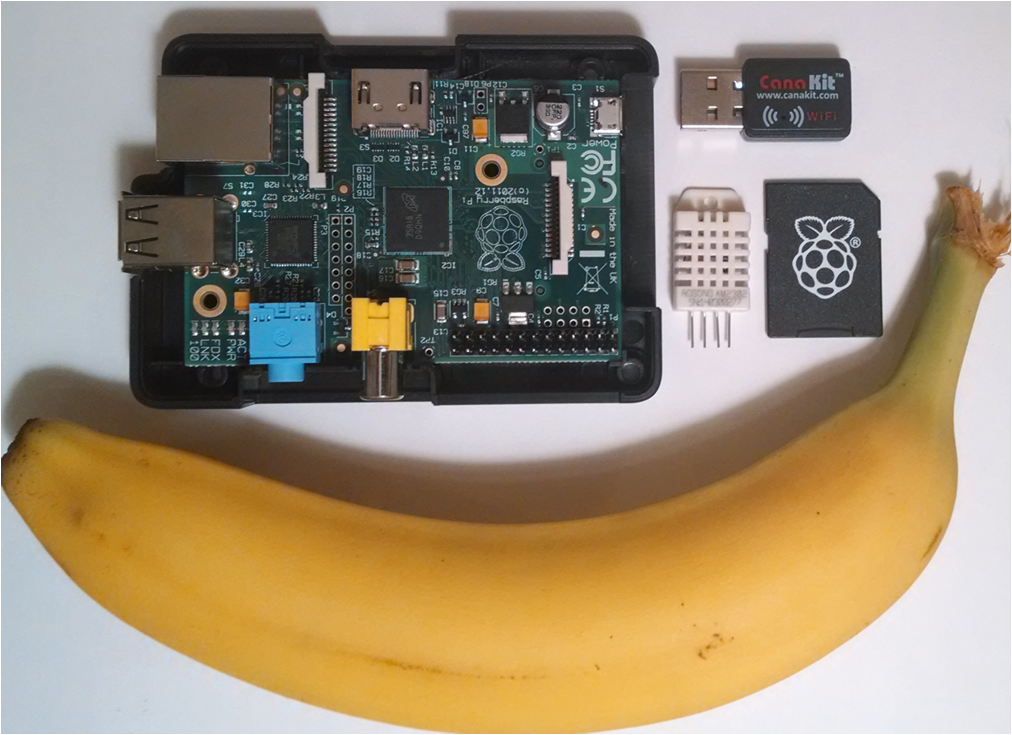
\includegraphics[scale=0.55]{disassembled.PNG}}
	\caption{Disassembled (Banana for Scale)}
\end{figure}
\begin{figure}[H]
	\makebox[\textwidth]{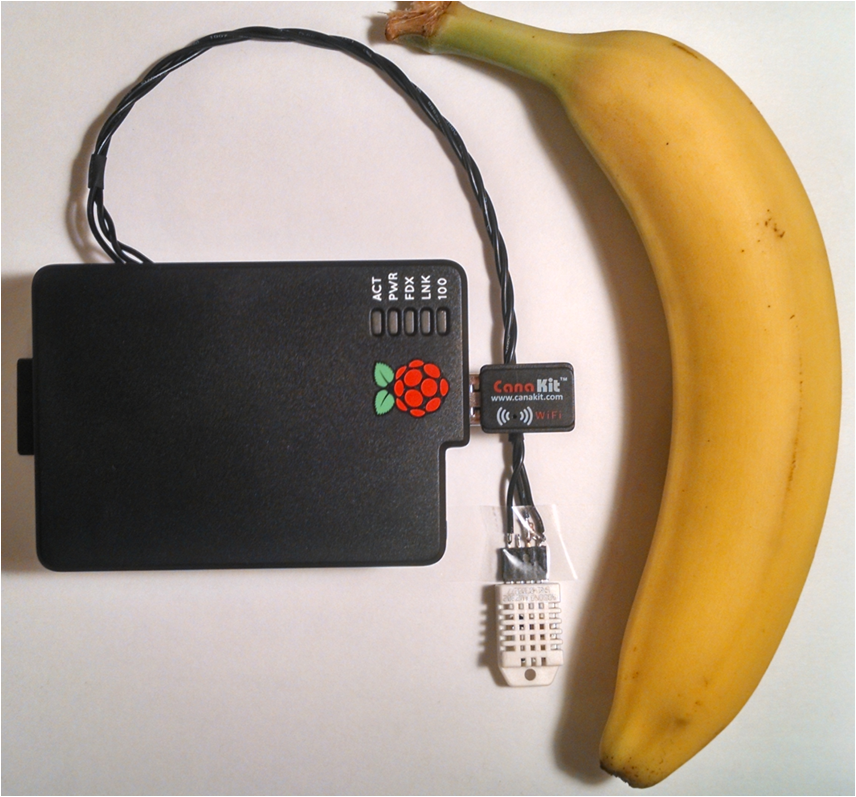
\includegraphics[scale=0.55]{assembled.PNG}}
	\caption{Assembled (Banana for Scale)}
\end{figure}
\newpage

\subsection*{Testing}
\addcontentsline{toc}{subsection}{Testing}
\indent
\indent
There are two types of testing that we used in this project: Unit Testing and Functional Testing. Unit Testing is a must because it will allow the user to test every feature when a new patch comes out and allows after each code change to check if the features still work. Unit tests cannot be used to check everything so there must also be functional tests that show the site is reacting correctly and can handle loads properly.
\newline
\indent
Unit tests for this project are run through the command line and use Laravel's testing framework. 
\begin{figure}[H]
	\makebox[\textwidth]{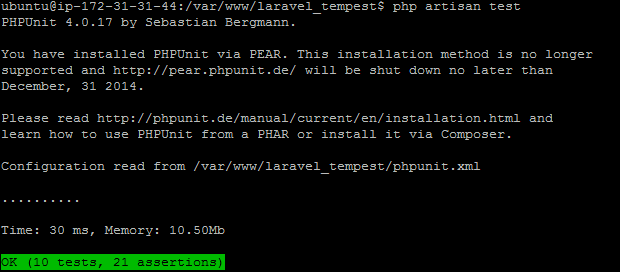
\includegraphics[scale=0.75]{test_pass.png}}
	\caption{Successful Running of Unit Tests}
\end{figure}
\indent
There were many different functional tests that we run to test the full functionality of our project. Some of the big functional tests that we run are for email alerts, text message alerts and virtual sensors.
\begin{figure}[H]
	\makebox[\textwidth]{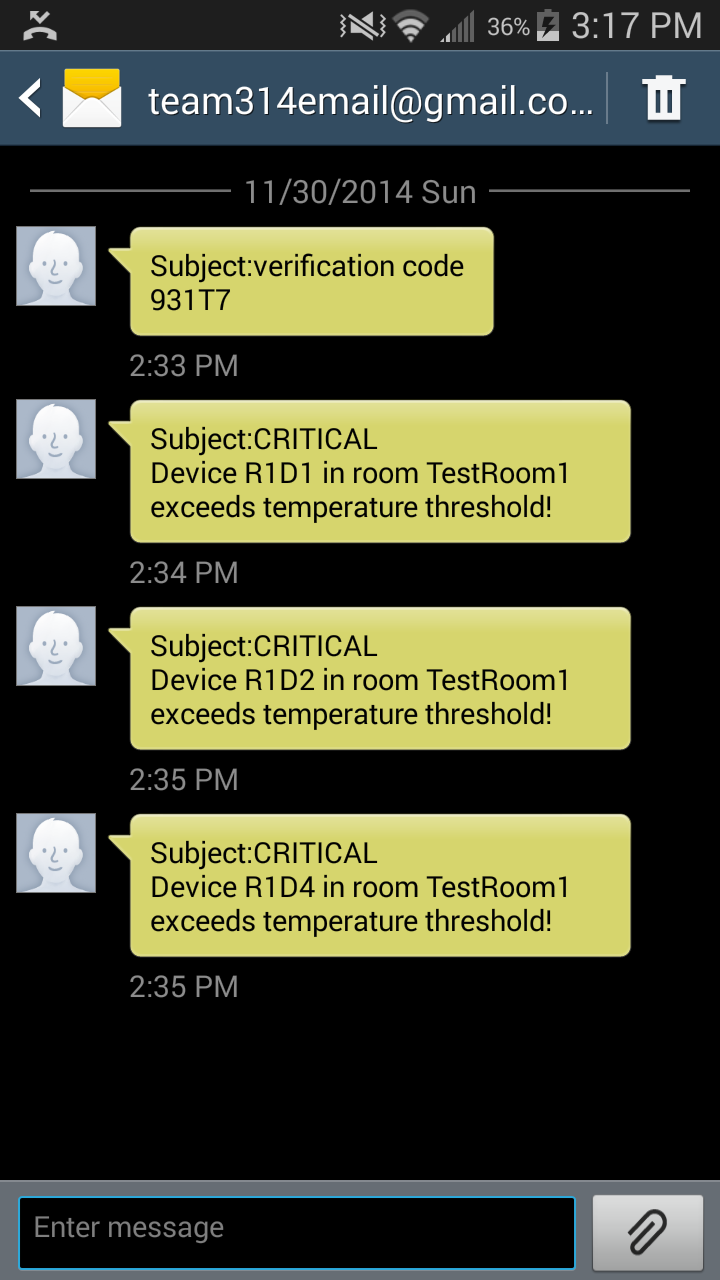
\includegraphics[scale=0.25]{textmessage.png}}
	\caption{Text Message Alert and Verification Functional Testing}
\end{figure}
\begin{figure}[H]
	\makebox[\textwidth]{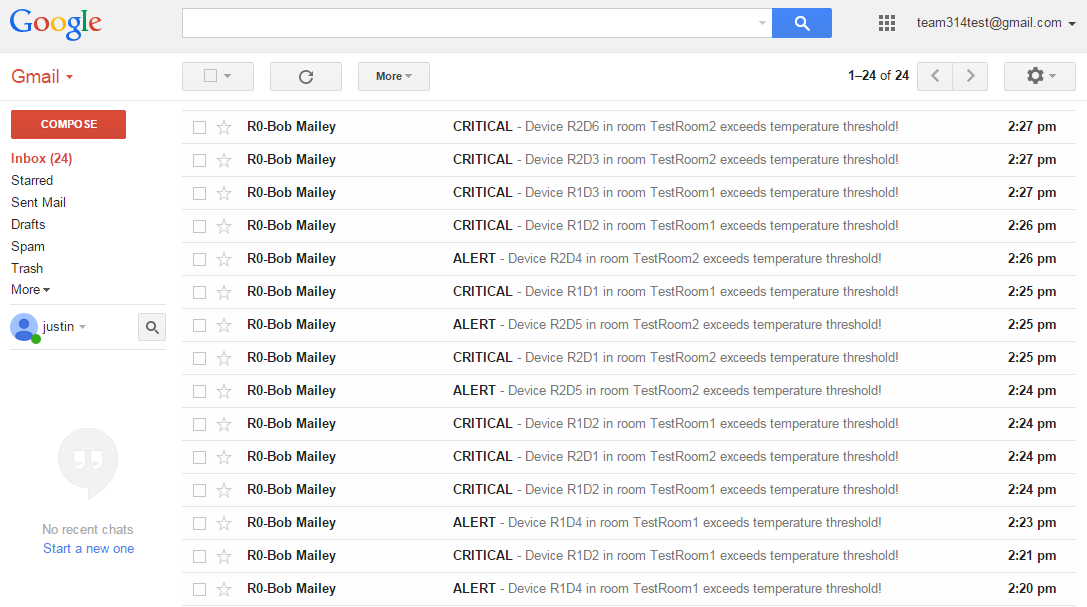
\includegraphics[scale=0.65]{emailalerts.png}}
	\caption{Email Alert Functional Testing}
\end{figure}
\begin{figure}[H]
	\makebox[\textwidth]{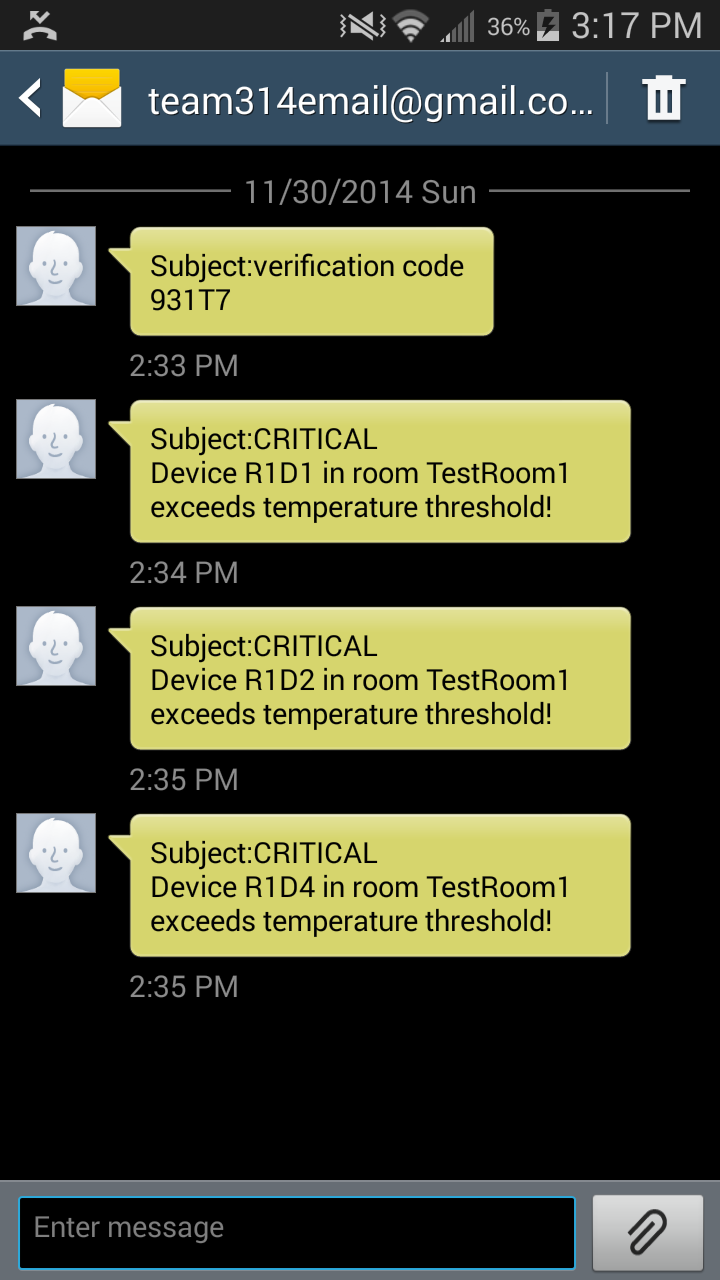
\includegraphics[scale=0.25]{textmessage.png}}
	\caption{Multiple Sensor Testing}
\end{figure}
\indent
We also used the sensor units we build to do functional testing. We put the units near hot and cold things like an oven or a refrigerator and measured the actual readings with a thermometer and humidity measuring device. We then checked the web site to make sure the sensor units were reporting accurate readings.
\newpage

\subsection*{Security}
\addcontentsline{toc}{subsection}{Security}
\indent
\indent
Security was a big concern of our Client. Used Laravel's industry-grade tools to create a secure website. Some of the things we used and prevented were:
\begin{itemize}
	\item Sessions
	\item Tokens
	\item Input Sanitization
	\item XSS
	\item SQL Injections
	\item Password Hashing
\end{itemize}
\indent
Each of these items is useful on their own, but used together, they are quite secure.
\newline
\indent
For sessions, we simply used Laravel's standard interface. This means session-hijacking can not be done. If the user logs out, hitting the back button will not magically log them back in. If the user is already signed in, then another device can not log in as that user.
\newline
\indent
Tokens are very important when trying to prevent false data. A token is basically a key that verifies the identity of the user or the sensor unit. By using tokens and the other security features, the only way a malicious person can infiltrate the website is by physically messing with the sensor unit hardware.
\newline
\indent
Input Sanitization is the key to making sure that malicious or bad information cannot enter the web site. By making sure the user cannot submit certain pieces of data if the data doesn't conform to a specification, we can prevent a malicious user from breaking the web site.

\newpage

\subsection*{Maintenance}
\addcontentsline{toc}{subsection}{Maintenance}
\indent
\indent
After the completion of this project the current senior design team will offer no maintenance. All modifications will be done by the staff at Western Michigan University and anyone else who uses the project. This being said there are modifications that we had planned but didn't have time to get to that could be added to increase the user experience for the project. These include
\begin{itemize}
	\item Adding a secure layer between the pi and the server,
	\item Adding historical data logging to the Raspberry Pi,
	\item Creating a way to retrieve historical data from the device if it was down for a period,
	\item Upgrading the user control area to have group administration,
	\item Making a program that would poll servers for their data and add it to a graph.
\end{itemize}
\indent
We plan on working on implementing these features, and modifying the project with our own ideas in the coming future, gut we do not guarantee any finished products. We will, however, offer our work to the client upon completion of a stable version and successful testing.
\newline
\indent
In addition, we have created multiple guides and how-to manuals for installing and building the sensor unit, and for putting the server together.
\newpage

\subsection*{Resources}
\addcontentsline{toc}{subsection}{Maintenance}

\begin{itemize}
	\item Raspberry Pi
	\item Temperature Sensor(s)
	\item Humidity Sensor(s)
	\item Externally Hosted Web Server
	\item Soldering Equipment
	\item Cabling to Connect Sensor to Pi
	\item Resistor
	\item SD card(s) loaded with the Raspbian Operating System
	\item Power Connector(s) for Raspberry Pi
	\item WiFi usb dongle for Raspberry Pi
\end{itemize}
\newpage

\subsection*{References}
\addcontentsline{toc}{subsection}{References}
For everything raspberry pi we use these sites
\begin{itemize}
	\item http://www.raspberrypi.org/
	\item http://www.raspbian.org/
	\item C Programming 2nd Edition
	\item http://www.adafruit.com/
\end{itemize}
For everything web server related these are the sites we use
\begin{itemize}
	\item http://laravel.com/docs/quick
	\item http://www.w3schools.com/
	\item http://www.noip.com
	\item http://httpd.apache.org/
	\item http://www.w3.org
	\item http://aws.amazon.com/
\end{itemize}
\newpage

\subsection*{Glossary}
\addcontentsline{toc}{subsection}{Glossary}
\begin{description}
	\item [GUI] \hfill \\
		Graphical User Interface. The windows a user interacts with.
	\item [MSP430 Launchpad] \hfill \\
		A 16-bit microcontroller platform made by Texas Instruments.
	\item [RaspberryPi] \hfill \\
		A credit-card-sized single-board computer developed by the Raspberry Pi Foundation.
	\item [Arduino] \hfill \\
		A series of microcontrollers that are very commonly used for computer to real world communications.
	\item [Raspbian] \hfill \\
		A Debian based operating system that we will use for our Raspberry Pi’s
	\item [CEAS] \hfill \\
		College of Engineering and Applied Sciences at Western Michigan University.
	\item [PHP] \hfill \\
		A recursive acronym for “PHP Hypertext Preprocessor” - the web programming language being used.
	\item [LAMP] \hfill \\
		LAMP is an acronym for Linux Apache Mysql PHP and is a common way to host dynamic websites
	\item [Apache] \hfill \\
		Apache is a web host used for serving up web pages all around the web.
\end{description}
\newpage

\subsection*{Ownership}
\addcontentsline{toc}{subsection}{Ownership}
\begin{description}
	\item [Licenses] \hfill \\
		Our project is under several licenses. PHP is a free, open source, software released under the PHP License. Laravel is licensed under the MIT license and per the agreement we are “free to modify, distribute and re-publish the source code on the condition that the copyright notices are left intact”. In the event that our project was used to generate revenue, or be sold as a standalone software package, the license permits us “to incorporate Laravel into any commercial or closed source application”. The GNU license for our project is open source and will be hosted for all to access and modify as they desire on GitHub.com.
	\item [Intellectual Property (IP)] \hfill \\
		As this project is being developed as a Senior Design project for Western Michigan University (WMU) under the direction of Dr. John Kapenga, WMU will retain the intellectual rights to the software.
	\item [Non-Disclosure Agreement (NDA)] \hfill \\
		No non-disclosure agreement is being used at this time. The project is maintained on GitHub.com, which is freely and openly accessible to anyone who wishes to view it, and is thus tracked by search engines such as Google, where it is able to be searched for by anyone on the planet.
	\item [Warranty] \hfill \\
		A maintenance document has been created for the project. Other than that document and this document no other outside assistance is required by the members of this project, and no warranty is given or implied.
\end{description}

\end{document}
